\documentclass[lineno]{jfm}

\usepackage{graphicx}
%\usepackage{epstopdf,epsfig}
\usepackage{newtxtext}
\usepackage{newtxmath}
\usepackage{natbib}
\usepackage{hyperref}
\usepackage{mathtools}
\usepackage{commath}
\usepackage{todonotes}
%
\usepackage[justification=justified]{caption}


\hypersetup{
    colorlinks = true,
    urlcolor   = blue,
    citecolor  = black,
}
\newtheorem{lemma}{Lemma}
\newtheorem{corollary}{Corollary}
\newcommand{\RomanNumeralCaps}[1]
\linenumbers


% Bryan's Marcros
\renewcommand{\aa}{\mathbf{a}}
\newcommand{\bd}{\partial}
\newcommand{\dd}{\mathbf{d}}
\newcommand{\DD}{\mathcal{D}}
\newcommand{\eeta}{\boldsymbol{\eta}}
\newcommand{\FF}{\mathbf{F}}
\newcommand{\GG}{\mathbf{G}}
\newcommand{\JJ}{\mathbf{J}}
\newcommand{\nnu}{\boldsymbol{\nu}}
\newcommand{\ttau}{\boldsymbol{\tau}}
\newcommand{\ssigma}{\boldsymbol{\sigma}}
\newcommand{\rr}{\mathbf{r}}
\newcommand{\RR}{\mathbf{R}}
\renewcommand{\SS}{\mathbf{S}}
\newcommand{\xx}{\mathbf{x}}
\newcommand{\XX}{\mathbf{X}}
\newcommand{\uu}{\mathbf{u}}
\renewcommand{\vv}{\mathbf{v}}
\newcommand{\yy}{\mathbf{y}}
\newcommand{\pderiv}[2]{\frac{\partial #1}{\partial #2}}
\newcommand{\jump}[1]{[\![ #1 ]\!]}


% {\MakeUppercase{\romannumeral #1}}

%\title{Two-Dimensional Vesicles Under External Flow via Integral Equation Method}
\title{Modeling Two-Dimensional Vesicle Hydrodynamics with Hydrophobic Attraction Potential Simulations}
%\author{Alan N. Jones\aff{1}
%  \corresp{\email{JFMEditorial@cambridge.org}},
%  H.-C. Smith\aff{1}
% \and J.Q. Long\aff{2}}
%
%\affiliation{\aff{1}STM Journals, Cambridge University Press, The Printing House, Shaftesbury Road, Cambridge CB2 8BS, UK
%\aff{2}DAMTP, Centre for Mathematical Sciences, Wilberforce Road, Cambridge CB3 0WA, UK}


\author{
Szu-Pei Fu\aff{1},
Bryan Quaife\aff{2},
Rolf Ryham\aff{1}, \and
Yuan-Nan Young\aff{3}
}
 \affiliation{
\aff{1}Department of Mathematics, \\Fordham University, Bronx, New York 10458, USA
\aff{2}Department of Scientific Computing, \\Florida State University, Tallahassee, Florida 32306, USA
\aff{3}Department of Mathematical Sciences, New Jersey Institute of Technology,\\ Newark, New Jersey 07102, USA
 }





\begin{document}
\maketitle

\begin{abstract}
  In this work, we study the dynamics of many-body systems immersed in a
  viscous fluid with a specified interparticle force. In particular, we
  apply a hydrophobic attraction potential (HAP) using a Janus type
  granular system to model lipid bilayer membranes. Coupling with an
  efficient integral equation method for rigid bodies in Stokes flow and
  a previous developed HAP solver, the deformations of a two-dimensional
  vesicle such as tank-treading motion and membrane ruptures can be
  observed under different values of the shear rate. Moreover, an
  efficient integral equation method is adopted for solving the screened
  Laplace equation and the mobility problem where it can accurately
  calculate hydrophobic and hydrodynamic interactions between near
  touched boundaries.
\end{abstract}


\begin{keywords}
Authors should not enter keywords on the manuscript, as these must be chosen by the author during the online submission process and will then be added during the typesetting process (see \href{https://www.cambridge.org/core/journals/journal-of-fluid-mechanics/information/list-of-keywords}{Keyword PDF} for the full list).  Other classifications will be added at the same time.
\end{keywords}

{\bf MSC Codes }  {\it(Optional)} Please enter your MSC Codes here



%%%%%%%%%%%%%%%%%%%%%%%%%%%%%%%%%%%%%%%%%%%%%%%%%%%%%%%%%%%%%%%%%%%%%%%
\section{\label{intro}Introduction}
Described by de Gennes as ``another animal in soft matter physics", the
Janus particle (often a spherical particle with a hydrophobic and a
hydrophilic hemisphere) exhibits complex aggregate, clustering, and
self-assembly into mesoscopic and macroscopic structures that are
relevant to a wide range of applications in biology and bioengineering.
Whether it is surface chemistry or polarity under an external field, the
dynamics of Janus particles is inevitably the combination of long-range
hydrodynamics interactions in the presence of short- and
intermediate-range particle-particle interactions. Recently~\cite{Fu20}
illustrated that the hydrophobic interactions between Janus particles in
a viscous solvent can be used as a coarse-grained model to capture the
mechanics of an elastic bilayer membrane of amphiphilic macromolecules
such as lipids. Depending on the total number of Janus particles and
their geometry, in a viscous solvent, Janus particles can aggregate to
form a micelle, a patch of bilayer membrane with open ends, and a
self-enclosed bilayer membrane (referred to as a JP vesicle). Using a
hybrid continuum model for the interactions between amphiphilic
particles in a viscous solvent and with a boundary integral
formulation,~\cite{Fu20} showed that the membrane granularity during
fusion and fission of bilayers can be accurately captured. 
%This boundary integral formulation has inspired more recent work

In molecular dynamics (MD) simulations, the lipid bilayer membranes are
often approximated by an implicit solvent coarse-grained model for
lipids (as in the Martini code), where their hydrodynamic interactions
are simplified by an implicit solvent. The long-range hydrodynamic
interactions and the induced long-range lipid interactions can be
captured by combining the Dry Martini with a lattice Boltzmann MD.
\cite{Brandner2019} used this methodology to simulate the hydrodynamics
of a nano-sized vesicle under a shear flow, and reproduced the well-know
vesicle hydrodynamics such as tank-treading, tumbling, and inter-leaflet
slippage (reported from simulations of the Helfrich-type continuum
model).

In this work we extend the hybrid continuum model in~\cite{Fu20} for the
Janus suspension to incorporate the collective hydrodynamics of a Janus
suspension under various flows: a linear shear flow, an elongation flow,
and a Poiseuille flow. We demonstrate that a JP vesicle behaves like
a vesicle in these flowing conditions. In particular, we show that a
JP vesicle undergoes tank-treading in a shear flow and vertical
migration in a Poiseuille flow. Furthermore we use the hybrid continuum
model to investigate the inter-leaflet slippage and rupture of a bilayer
membrane due to an imposed flow. Finally, we compare a pair of
interacting JP vesicles with a continuum model of a pair of vesicles.

We require a numerical method to avoid unphysical contact between rigid
Janus particles. Optimization-based contact methods introduce
constraints, such as enforcing a non-positive space-time interference
volume (\cite{lu-rah-zor2017, Lukas19, yan-cor-mal-vee-she2020}). These
methods do not introduce stiffness, but potentially expensive nonlinear
complementarity problems must be solved at each time step.
Repulsion-based contact methods, which we employ, introduce an
artificial repulsion force that increases in strength as two particles
approach one another (\cite{glo-pan-hes-jos-per2001, fen-mic2004,
kab-qua-bir2018}). Strong repulsion forces can introduce numerical
stiffness, but with the presence of the hydrophobic forces, we maintain
contact-free suspensions with a relatively weak non-stiff repulsive
force.

This paper is organized as follows. In \S~\ref{sec:governing_eqs} we
present the formulation for the Janus particles in a viscous fluid in
the zero-Reynolds number regime. In \S~\ref{sec:IEM} we extend the
hybrid continuum model for a Janus suspension to include the effects of
a far-field flow via the mobility problem formulation. In
\S~\ref{results} we validate our model and present simulation results
for a single and pair of JP vesicles under various flowing conditions.
Finally we provide discussion and outlook for future directions in
\S~\ref{conclusion}.

%%%%%%%%%%%%%%%%%%%%%%%%%%%%%%%%%%%%%%%%%%%%%%%%%%%%%%%%%%%%%%%%%%%%%%%
\section{Governing Equations\label{sec:governing_eqs}}
\subsection{\label{mobility}Mobility Problem}
We consider an $N_b$-many body collection of Janus particles suspended
in a two-dimensional unbounded domain $\Omega$. The boundary of each
particle is denoted by $\Gamma_i$ so that $\bd \Omega = \Gamma_1 \cup
\Gamma_2 \cup \cdots \cup \Gamma_{N_b}$. Assuming the inertial terms are negligible, the
governing equations are
\begin{alignat}{3}
  -\mu \Delta \uu + \nabla p &= \mathbf{0}, 
    && \xx \in \Omega, \\
  \nabla\cdot \uu &= 0, \qquad && \xx \in \Omega, \\
  \uu - \uu_\infty &\to \mathbf{0}, && |\xx| \to \infty,
\end{alignat}
%
where $\uu$ is the velocity, $\mu$ is the constant viscosity, $p$ is the
pressure, and $\uu_\infty$ is the background flow. Since each particle
$\Gamma_i$ with center $\aa_i$ is a rigid body, its velocity satisfies 
\begin{align}
  \vv(\xx) = \vv_i + \omega_i (\xx - \aa_i)^\perp, \quad 
    \xx \in \Gamma_i,
\end{align}
where $\vv_i$ is its translational velocity and $\omega_i$ is its
angular velocity. Here, $\langle x, y \rangle^{\perp} = \langle -y, x
\rangle$. Therefore, the no-slip boundary condition on each particle is
\begin{align}
  \uu(\xx) = \vv_i + \omega_i (\xx - \aa_i)^\perp, \quad
    \xx \in \Gamma_i.
\end{align}
To determine the translational and angular velocities of each particle,
we define imposed forces $\FF_i$ and torques $T_i$ acting on each
particle. Since the small particles are intertialess, force balance
gives 
\begin{alignat}{2}
  \label{eq:force}
  \FF_i &+ \int_{\Gamma_i} \ssigma \cdot \nnu_i \, \dif s = \mathbf{0},
  && i=1,\ldots,N_b,\\
  \label{eq:torque}
  T_i &+ \int_{\Gamma_i} (\xx - \aa_i)^\perp \cdot 
    (\ssigma \cdot \nnu_i) \, \dif s = 0, \qquad && i=1,\ldots,N_b,
\end{alignat}
where $\ssigma = -p \mathbf{I} + \mu \left(\nabla \uu + \nabla \uu^T
\right)$ is the hydrodynamic stress tensor (pressure tensor) and
$\nnu_i$ is the particle outward normal. The process of finding the
translational and angular velocities given the forces and torques is
referred to as the mobility problem.


%%%%%%%%%%%%%%%%%%%%%%%%%%%%%%%%%%%%%%%%%%%%%%%%%%%%%%%%%%%%%%%%%%%%%%%
\subsection{Imposed Forces}
The imposed forces and torques contain two parts. The first part comes
from the hydrophobic attraction potential (HAP). This potential was
introduced in~\cite{Fu20} and models hydrophobic attraction by solving
the screened Laplace equation boundary value problem
\begin{alignat}{2}
  \label{eq:SL}
-\rho^2 \Delta u + u &=0,            && \xx \in \Omega,\\
\label{eq:SLbc}
u(\xx) &= f_i(\xx),\qquad  && \xx \in \Gamma_i,\; i=1,\ldots,N_b \\
\label{eq:SLff}
u &\to 0,                          &&|\xx| \to \infty,
\end{alignat}
where $0 \leq f_i \leq 1$ is a material label with $f_i = 0$,
respectively $1$, representing hydrophilic, respectively hydrophobic,
portions of the surface. We assume that the $f_i$ and $\Gamma_i$ are
smooth. The parameter $\rho$ is the decay length of attraction. The
forces and torques for this attraction are 
\begin{align}
  \label{eq:hydrophobicAttraction}
  \FF_i^{\text{hydro}} = \int_{\Gamma_i} {\bf T}\cdot \nnu_i \, \dif s, 
    \quad 
  T_i^{\text{hydro}} = \int_{\Gamma_i} (\xx - \aa_i)^{\perp} \cdot ({\bf T} \cdot \nnu_i) \dif s,
\end{align}
where
\begin{align}
  \label{eq:stress}
\mathbf{T}
= \gamma\rho^{-1}u^2 \mathbf{I} + 2\rho\gamma \left(\tfrac{1}{2}|\nabla
  u|^2 \mathbf{I} - \nabla u  \nabla u^T\right)
\end{align}
is the hydrophobic stress tensor. The parameter $\gamma$ is
the interfacial
tension. The forces $\FF_i^{\text{hydro}}$ and torques
$T_i^{\text{hydro}}$ are responsible for forming particle aggregates
that partially sequester the hydrophobic portions of the particle
surface.

The second part of the imposed forces and torques comes from repulsion
between proximal particles. Given a pair particles indexed with $i$ and
$j$, we find the two points $\tilde{\xx}_i \in \Gamma_i$ and
$\tilde{\xx}_j \in \Gamma_j$ that are closest to one another. We then
define the repulsion force and torque
\begin{align}
  \label{eq:REPULforce}
  \FF_i^{\text{repul}} &= \sum_{j \neq i} 
    \frac{\tilde{\xx}_i - \tilde{\xx}_j}
    {|\tilde{\xx}_i - \tilde{\xx}_j|} 
    P'(|\tilde{\xx}_i - \tilde{\xx}_j|), \\
  \label{eq:REPULtorque}
  T_i^{\text{repul}} &= \sum_{j \neq i} 
    (\tilde{\xx}_i - \aa_i)^{\perp} \cdot 
    \frac{\tilde{\xx}_i - \tilde{\xx}_j}
    {|\tilde{\xx}_i - \tilde{\xx}_j|} 
    P'(|\tilde{\xx}_i - \tilde{\xx}_j|).
\end{align}
The repulsion profile $P(r)$ is zero for distances $r$ larger than a
repulsion length scale $\rho_0$. As such,~\eqref{eq:REPULforce}
and~\eqref{eq:REPULtorque} ignore particles $\Gamma_j$ outside a
tubular neighborhood of $\Gamma_i$. For $0 \leq r < \rho_0,$ we use
$P(r) = M(1 - \sin(r/\rho_0))$ where $M$ is sufficiently large to
prevent particle collisions. Then, the total imposed force and torque
are
\begin{align}
  \FF_i = \FF_i^{\text{hydro}} + \FF_i^{\text{repul}},\quad
  T_i = T_i^{\text{hydro}} + T_i^{\text{repul}}, \qquad
  i=1,\ldots,N_b.
\end{align}


%%%%%%%%%%%%%%%%%%%%%%%%%%%%%%%%%%%%%%%%%%%%%%%%%%%%%%%%%%%%%%%%%%%%%%%
\subsection{Time Marching}
By solving the mobility problem, we obtain translational and angular
velocities of the $N_b$-body system. A second-order Adams-Bashforth
scheme updates the particle positions and orientations. By including the
repulsion force~\eqref{eq:REPULforce} and
torque~\eqref{eq:REPULtorque}, particle collisions are avoided even
when using a relatively large time step. 



%This paper is organized as follows. Chapter 2 introduces the mobility problem..... The integral equation method for solving $N_b$-body system with details of .... are included in Chapter 3. We provide numerical results of vesicle simulations in Chapter 4. Finally, we conclude the work and briefly give the picture of our future work.



%%%%%%%%%%%%%%%%%%%%%%%%%%%%%%%%%%%%%%%%%%%%%%%%%%%%%%%%%%%%%%%%%%%%%%%
\section{Integral Equation Method}
\label{sec:IEM}
Computing the hydrophobic attraction potential and the particle forces
and torques requires the solution of elliptic partial differential
equations (PDEs) in an unbounded complex domain. We recast both these
PDEs as boundary integral equations (BIEs). We discretize each BIE at
$N$ points on each of the $N_b$ particles with a collocation method.
Integrals that are smooth are computed with the spectrally-accurate
trapezoid rule, and nearly-singular integrals, caused by close contact
between two particles, are computed with a high-order
interpolation-based quadrature rule (\cite{qua-bir2014}). After
discretizing and applying quadrature, the resulting linear system is
solved with matrix-free GMRES, and we guarantee that the number of GMRES
iterations is mesh-independent by using second-kind BIEs.


%%%%%%%%%%%%%%%%%%%%%%%%%%%%%%%%%%%%%%%%%%%%%%%%%%%%%%%%%%%%%%%%%%%%%%%
\subsection{HAP Boundary Integral Equation}
Similar to our previous work (\cite{Fu20}), we represent the HAP as a
double-layer potential
\begin{align}
  \label{eq:HAP_DLP}
  u(\xx) = \frac{1}{2\pi} \int_{\bd\Omega} \pderiv{}{\nnu_\yy}
    K_0 \left(\frac{|\xx - \yy|}{\rho}\right) \sigma(\yy) \, \dif s_\yy,
    \quad \xx \in \Omega,
\end{align}
where $K_0$ is the zeroth-order modified Bessel function of the first
kind and the integral is taken in the sense of principle value whenever $\xx \in \partial \Omega$. 
By requiring that the density function $\sigma$ satisfies the
second-kind integral equation
\begin{equation}
\label{eq:screenedSKIE}
  f(\xx) = \frac{1}{2}\sigma(\xx) + 
    \frac{1}{2\pi}\int_{\bd\Omega} \pderiv{}{\nnu_\yy}
    K_0 \left(\frac{|\xx - \yy|}{\rho}\right) \sigma(\yy) \, \dif s_\yy,
    \quad \xx \in \bd\Omega,
\end{equation}
the HAP double-layer potential~\eqref{eq:HAP_DLP} satisfies the screened
Laplace equation~\eqref{eq:SL}--\eqref{eq:SLff}. After
discretizing~\eqref{eq:screenedSKIE}, the result is a $NN_b \times NN_b$
linear system that is solved with block-diagonal preconditioned GMRES.

To calculate the hydrophobic force and torque, the gradient of the
double-layer potential~\eqref{eq:HAP_DLP} must be computed on the
boundary of each particle. The resulting integrands are singular, and
specialized quadrature would be necessary to approximate such integrals.
Alternatively, in Section~\ref{subsec:calculating_force}, we show that
the force and torque calculations can be expressed in terms of
non-singular integrals.

%%%%%%%%%%%%%%%%%%%%%%%%%%%%%%%%%%%%%%%%%%%%%%%%%%%%%%%%%%%%%%%%%%%%%%%
\subsection{Mobility Problem Boundary Integral Equation}
Following previous work of~\cite{Lukas19}, we use the velocity
representation of~\cite{pow-mir1987}. In particular, we write the
velocity as the sum of a double-layer potential and $N_b$ Stokeslets and
Rotlets
\begin{align}
  \label{eq:velocity}
  \uu(\xx) = \uu_\infty(\xx) + \DD[\eeta](\xx) + 
    \sum_{i=1}^{N_b} \left(\SS(\xx,\aa_i) \FF_i + 
    \RR(\xx,\aa_i) T_i\right), \quad \xx \in \Omega.
\end{align}
The double-layer potential is
\begin{align}
  \DD[\eeta](\xx) = \frac{1}{\pi} \int_{\bd\Omega} 
    \frac{\rr \cdot \nnu}{\rho^2} \frac{\rr \otimes \rr}{\rho^2}
    \eeta(\yy) \, \dif s_\yy,
\end{align}
where $\rr = \xx - \yy$ and $\rho = |\rr|$. The Stokeslet and Rotlet
centered at $\aa_i$ are
\begin{align}
  \SS(\xx,\aa_i)\FF_i &= \frac{1}{4\pi} \left(-\log \rho + 
    \frac{\rr \otimes \rr}{\rho^2}\right) \FF_i, \\
  \RR(\xx,\aa_i)T_i &= \frac{1}{4\pi} \frac{\rr^\perp}{\rho^2} T_i,
\end{align}
respectively, where $\rr = \xx - \aa_i$ and $\rho = |\rr|$. The
Stokeslet is torque-free and has force $\FF_i$ while the Rotlet is
force-free and has torque $T_i$. Therefore, the
velocity~\eqref{eq:velocity} satisfies the total force~\eqref{eq:force}
and torque~\eqref{eq:torque} conditions if the double-layer potential
$\DD[\eeta]$ is force- and torque-free.  Matching the limit
of~\eqref{eq:velocity} with the rigid body motion, and imposing that
$\DD[\eeta]$ is force- and torque-free, the density function $\eeta$,
translational velocity $\vv_i$, and angular velocity $\omega_i$ satisfy
\begin{alignat}{3}
  \nonumber
  \vv_i + \omega_i (\xx - \aa_i)^\perp &= \uu_\infty(\xx)
    -\frac{1}{2} \eeta(\xx) + \DD[\eeta](\xx) \\
  \label{eq:SKIE}
    + \sum_{j=1}^{N_b} &
    \left(\SS(\xx,\aa_j) \FF_j + \RR(\xx,\aa_j) T_j\right),
    \quad &&\xx \in \Gamma_i,\: i=1,\ldots,N_b, \\
  \label{eq:mobility1}
  \int_{\bd\Gamma_i} \eeta \cdot \nnu_i \, \dif s &= {\bf 0}, 
  &&i = 1,\ldots,N_b, \\
  \label{eq:mobility2}
  \int_{\bd\Gamma_i} \eeta\times(\xx-\aa_i)^\perp \cdot \nnu_i \, \dif s &= 0,
  &&i = 1,\ldots,N_b.
\end{alignat}

After discretizing and applying appropriate quadrature rules, the result
is a $(2NN_b + 3N_b) \times (2NN_b + 3N_b)$ linear system that we solve
with block-diagonal preconditioned GMRES. We note that other BIE
formulations of the mobility problem use single-layer potentials
(\cite{cor-gre-rac-vee2017, rac-gre2016}) or a combination of single-
and double-layer potentials (\cite{cor-vee2018}).

We validated our solver for \eqref{eq:SKIE}-\eqref{eq:mobility2} using a
single elliptical particle suspended in a background shear flow (see \S
\ref{sec:ves_in_shear}). Hydrophobic attraction and repulsion are zero
for a single particle. The angle of the ellipse's major axis coming from
the integral equation method was in complete agreement with the
theoretical, Jeffrey oribit time-course \cite{}. 
  
%The Jeffrey orbit  
%\begin{equation}
%\label{eq:jeff}
%\Theta(t) = \tan^{-1}\left(\frac{a}{b}\tan \left(\frac{ab \dot\gamma t}{a^2+b^2}\right)\right)
%\end{equation}
%gives the angle between the major axis and $\mathbf{e}_2$
%where $a$, $b$ are the semi-major and semi-minor axes. 
%We are assuming $\Theta(0) = 0$.
% 

%The background flow is a shear flow $\uu_{\infty}(\xx) = \dot\gamma  \xx \cdot \mathbf{e}_2 \mathbf{e}_1$ with shear rate $\dot\gamma$
%and orthogonal unit vectors $\mathbf{e}_1$ and $\mathbf{e}_2$. 
%A single elliptical particle is suspended in the fluid with center at the origin.
%The Jeffrey orbit  
%\begin{equation}
%\label{eq:jeff}
%\Theta(t) = \tan^{-1}\left(\frac{a}{b}\tan \left(\frac{ab \dot\gamma t}{a^2+b^2}\right)\right)
%\end{equation}
%gives the angle between the major axis and $\mathbf{e}_2$
%where $a$, $b$ are the semi-major and semi-minor axes. 
%We are assuming $\Theta(0) = 0$.
%Figure~\ref{figure1} shows that the angles coming from the integral equation method \eqref{eq:SKIE}-\eqref{eq:mobility2}
%are in complete agreement with the theoretical time course \eqref{eq:jeff}.  Hydrophobic attraction and repulsion are zero for a single particle. 

%%%%%%%%%%%%%%%%%%%%%%%%%%%%%%%%%%%%%%%%%%%%%%%%%%%%%%%%%%%%%%%%%%%%%%%
\subsection{Calculating the Hydrophobic Force}
\label{subsec:calculating_force}
Once \eqref{eq:screenedSKIE} has been solved for $\sigma$, we need to
evaluate the integrals~\eqref{eq:hydrophobicAttraction} which are the
HAP forces and torques. These integrals involve the
stress~\eqref{eq:stress} which contains a singular integral for the
gradient of the double-layer potential. To avoid singular integrals, we
first define
\begin{align}
  \label{eq:uidef}
  v_i(\xx) = u(\xx) - u_i(\xx),
\end{align}
where
\begin{align}
  u_i(\xx) &= \frac{1}{2\pi} \int_{\Gamma_i} \pderiv{}{\nnu_\yy}
    K_0 \left(\frac{|\xx - \yy|}{\rho}\right) \sigma(\yy) \, \dif s_\yy,
    \quad \xx \in \mathbb{R}^2.
\end{align}
That is, $v_i(\xx)$ is the double-layer potential~\eqref{eq:HAP_DLP}
with $\Gamma_i$ excluded from $\bd\Omega$. Having defined $v_i$, we can
show that
\begin{align}
  \label{eq:recipforcetorque}
  \FF_i^{\text{hydro}} = \int_{\Gamma_i} \JJ_i \,\dif s,\quad
  T_i^{\text{hydro}}    = \int_{\Gamma_i} 
    (\xx - \aa_i)^{\perp} \cdot \JJ_i  \,\dif s,
\end{align}
where
\begin{align}
  \label{eq:jumpstress1}
  \JJ_{i} = 2\gamma\rho^{-1} \sigma v_i \nnu + 
    2\gamma\rho \frac{d\sigma}{ds} \frac{dv_i}{ds} \nnu -
    2\gamma\rho \frac{d\sigma}{ds} \frac{dv_i}{d\nnu} \ttau.
\end{align}
Here, $\ttau$ and $\frac{d}{ds}$ are the unit tangent and arc length
derivative for $\Gamma_i$, respectively, and $\nnu$ is the unit normal.
The advantage in using~\eqref{eq:recipforcetorque} over
using~\eqref{eq:hydrophobicAttraction} is that the components $\sigma$,
$v_i$, $\frac{d\sigma}{ds}$, and $\frac{dv_i}{ds}$ of $\JJ_i$ are smooth
functions, whereas the components of \eqref{eq:stress} are singular
integrals. 

%To avoid singular integrals, we
%evaluate~\eqref{eq:hydrophobicAttraction} using the identities
%\begin{align}
%  \label{eq:recipforcetorque}
%  \FF_i^{\text{hydro}} = \int_{\Gamma_i} \JJ_i \,\dif s,\quad
%  T_i^{\text{hydro}}    = \int_{\Gamma_i} 
%    (\xx - \aa_i)^{\perp} \cdot \JJ_i  \,\dif s,
%\end{align}
%where
%\begin{align}
%  \label{eq:jumpstress1}
%  \JJ_{i} = 2\gamma\rho^{-1} \sigma v_i \nnu + 
%    2\gamma\rho \frac{d\sigma}{ds} \frac{dv_i}{ds} \nnu -
%    2\gamma\rho \frac{d\sigma}{ds} \frac{dv_i}{d\nu} \ttau.
%\end{align}
%Here, $\ttau$ and $\frac{d}{ds}$ are the unit tangent  and arc length
%derivative for $\Gamma_i$, respectively, and
%\begin{equation}
%\label{eq:uidef}
%\begin{aligned}
%    u(\xx) &= u_i(\xx) + v_i(\xx),\\
%    u_i(\xx) &= \frac{1}{2\pi} \int_{\Gamma_i} \pderiv{}{\nnu_\yy}
%    K_0 \left(\frac{|\xx - \yy|}{\rho}\right) \sigma(\yy) \, \dif s_\yy,
%    \quad \xx \in \mathbb{R}^2.
%\end{aligned}
%\end{equation}
%That is, $v_i(\xx)$ is the double-layer potential~\eqref{eq:HAP_DLP} with 
%$\Gamma_i$ excluded from $\bd\Omega$. The advantage in
%using \eqref{eq:recipforcetorque} over using \eqref{eq:hydrophobicAttraction} is that the components
%$\sigma$, $v_i$, $\frac{d\sigma}{ds}$, and $\frac{dv_i}{ds}$ of $\JJ_i$ are smooth functions,
%whereas the components of \eqref{eq:stress} are singular integrals.  

To prove \eqref{eq:recipforcetorque}, let 
\begin{align*}
  {\bf T} &=
    \mathbf{S}(u_i,u_i)
  +(\mathbf{S}(u_i,v_i)
  +\mathbf{S}(v_i,u_i))
  +\mathbf{S}(v_i,v_i) \\
  &= {\bf T}_1 + {\bf T}_2 + {\bf T}_3
\end{align*}
where we introduce the bilinear form
\begin{equation}
\label{eq:Tsplit}
\mathbf{S}(u,v)
=  \gamma\rho^{-1} uv {\bf I} + \gamma\rho \nabla u \cdot \nabla v {\bf I} - 2 \gamma \rho \nabla u \nabla v^T .
\end{equation}
Using the fact that $u$,  $u_i$, and $v_i$ solve the screened Laplace
equation~\eqref{eq:SL},  and that $\mathbf{T}$, $\mathbf{T}_j$, $j = 1,
2, 3$ are symmetric, it is straightforward to verify that 
  \begin{equation}
    \label{eq:decompdivfree}
    \nabla \cdot {\bf T}_j = 0, \quad
    \nabla \cdot ((\xx-\aa_i)^{\perp} \cdot {\bf T}_j) = 0, \quad j = 1, 2, 3.
  \end{equation}

%\begin{lemma}
%  \label{eq:stress_div_lemma}
%  \begin{equation}
%    \label{eq:decompdivfree}
%    \nabla \cdot {\bf T}_j = 0, \quad
%    \nabla \cdot (\xx^{\perp} \cdot {\bf T}_j) = 0
%  \end{equation}
% for  $ j = 1, 2, 3$.
%\end{lemma}
%\begin{proof}
%  Let $\mathbf{T}$ be as in \eqref{eq:stress}.  
%  It is straightforward to show that  
%%  \begin{align*}
% %   (\nabla \cdot {\bf T})_j &=
% %   \nabla_k   T_{jk}  = 0\\
% %   &= \rho^{-1} 2u \nabla_j u + \rho(2\nabla_{kl}^2 u \nabla_l u  - 2 \nabla_{kj}^2 u \nabla_k u
% %  - 2 \nabla_j u \nabla_{kk}^2 u )\\
% %   &=2\rho^{-1}(-\rho^2 \Delta u + u)\nabla_j u = 0,
% % \end{align*}
% \begin{equation*}
%\nabla \cdot {\bf T} = 2\rho^{-1}(-\rho^2 \Delta u + u)\nabla u = 0
% \end{equation*}
% since $u$ solves $-\rho^2 \Delta u + u = 0$.
% Moreover,
%  \begin{align*}
%    \nabla \cdot (\xx^{\perp} \cdot {\bf T} )
%%    &= \nabla_k (\epsilon_{jml}x_m T_{lk})\\
%%    &= \varepsilon_{jml} T_{lm} + \varepsilon_{jml}x_m \nabla_k T_{lk}\\
%%   &= (\boldsymbol{\varepsilon}:{\bf T} + {\bf x}^{\perp} \cdot \nabla \cdot {\bf T})_j.
%=  \mathbf{S}:\mathbf{T} + \mathbf{S}\xx \cdot (\nabla \cdot \mathbf{T}) = 0,
%  \end{align*}
%  since ${\bf T}$ is symmetric, where $\mathbf{S}\xx = \xx^{\perp}$.
%  
%  The functions $u_i$ and $v_i$ also solve the equation $-\rho^2 \Delta u + u = 0$.  Repeating the above argument 
%  for ${\bf T}_1 = \sigma[u_i,u_i]$ and ${\bf T}_3 = \sigma[v_i,v_i]$ gives that 
%  \eqref{eq:decompdivfree} holds for the cases $j = 1$ and $j = 3$. Finally,
%  \eqref{eq:decompdivfree} holds for the case $j = 2$ because
%  ${\bf T}_2 = {\bf T} - {\bf T}_1 - {\bf T}_3$.
%\end{proof}

Let $U_i$ be the interior of the particle indexed by $i$. For $\xx_0
\in \Gamma_i$ and an arbitrary function $g(\xx)$, the notation
\begin{align}
  \jump{g}(\xx_0) = \lim_{\substack{\xx \to \xx_0 \\ \xx \in U_i^c}}g(\xx)  - 
                    \lim_{\substack{\xx \to \xx_0 \\ \xx \in U_i}}g(\xx),
\end{align}
denotes the jump of the limits of $g(\xx)$ taken from the outside to
the inside of $\Gamma_i$.
%\begin{align}
%\lim_{\xx \to \xx_0^+}g(\xx),\quad 
%\lim_{\xx \to \xx_0^-}g(\xx), \quad
%  \jump{g}(\xx_0) = \lim_{\xx \to \xx_0^+}g(\xx)  - \lim_{\xx \to \xx_0^-}g(\xx)
%\end{align}
%denotes the limit taken from points in $U_i^c$,  the limit taken from
%points in $U_i$, and the jump, respectively.  
\begin{lemma}
\begin{align}
  \label{eq:prejump}
  \FF_i = \int_{\Gamma_i} \jump{{\bf T}_2  \nnu}  \, \dif s,\quad
  T_i = \int_{\Gamma_i} (\xx - \aa_i)^{\perp} \cdot \jump{{\bf T}_2 \nnu} \, \dif s.
\end{align}
\end{lemma}
\begin{proof}
To show~\eqref{eq:prejump}, we expand
\begin{align}
  \FF_i = \int_{\Gamma_i} {\bf T}_1\nnu + 
    {\bf T}_2\nnu + {\bf T}_3\nnu\,\dif s.
\end{align}
By~\eqref{eq:uidef} and~\eqref{eq:decompdivfree}, we have that $u_i$ is
smooth and $\nabla \cdot {\bf T}_1 = \mathbf{0}$ in $\mathbb{R}^n
\setminus U_i$. Similarly, $v_i = u - u_i$ is smooth and $\nabla \cdot
{\bf T}_3 = \mathbf{0}$ in $U_i$. By the divergence theorem,  
\begin{align}
  \int_{\Gamma_i}  {\bf T}_1\nnu \,\dif s
  = -\int_{\mathbb{R}^n \setminus U_i} \nabla \cdot {\bf T}_1 \,\dif \xx = \mathbf{0},\quad
    \int_{\Gamma_i}  {\bf T}_3 \nnu\,\dif s
  = \int_{U_i} \nabla \cdot {\bf T}_3 \,\dif \xx = \mathbf{0}.
\end{align}
Finally, $u_i$ and $v_i$ are smooth and $\nabla \cdot {\bf T}_2= 0$ in $U_i$. This gives
\begin{align}
  \mathbf{0} = \int_{U_i} \nabla \cdot {\bf T}_2 \, \dif \xx = -\int_{\Gamma_i}  
    ({\bf T}_2 \nnu)^-\,\dif s,
\end{align}
where the superscript denotes the limit taken from in $U_i$.  
Combining the previous four equations gives the first equation in \eqref{eq:prejump}.
The argument for the second equation in \eqref{eq:prejump} is identical. 
\end{proof}

We have the following jump relations for \eqref{eq:uidef}: 
\begin{equation}
\label{eq:DLjump}
\jump{u_i} = \sigma, \quad
\jump{v_i} = 0, \quad
\jump{\nabla u_i} = \frac{\dif \sigma}{\dif s}\ttau,\quad
\jump{\nabla v_i} = \mathbf{0},
\end{equation}
on $\Gamma_i$. Therefore,
\begin{align*}
  \jump{{\bf T}_2\nnu}   &= \jump{\mathbf{S}(u_i,v_i)\nnu  +\mathbf{S}(v_i,u_i)\nnu} \\
  &= \jump{( 2\gamma\rho^{-1} u_i v_i \mathbf{I} + 2\gamma\rho \nabla u_i \cdot \nabla v_i \mathbf{I} 
- 2\gamma\rho \nabla u_i  \nabla v_i^T - 2\gamma\rho \nabla v_i \nabla u_i^T)  \nnu}\\
&= 2\gamma\rho^{-1} \sigma v_i \nnu + 2\gamma\rho \frac{d\sigma }{ds}\frac{dv_i }{ds} \nnu
- 2\gamma\rho \ \frac{d\sigma }{ds} \frac{dv_i }{d\nu} \ttau = \JJ_i.
\end{align*}
Combing this with~\eqref{eq:prejump} gives~\eqref{eq:recipforcetorque}
as required. 



%%%%%%%%%%%%%%%%%%%%%%%%%%%%%%%%%%%%%%%%%%%%%%%%%%%%%%%%%%%%%%%%%%%%%%%
\section{\label{results}Numerical Results}

%%%%%%%%%%%%%%%%%%%%%%%%%%%%%%%%%%%%%%%%%%%%%%%%%%%%%%%%%%%%%%%%%%%%%%%

\subsection{Model Parameters}
To extract physical quantities of the target structure, we select
particles that are disks with diameter $l_0 = 2.5$ nm representing the
characteristic thickness of monolayers. The boundary
conditions~\eqref{eq:SLbc} are $f_i(\xx) = \tfrac{1}{2}(1 + \cos
\theta_i)$ where $\theta_i$ is the angle between $\xx - \aa_i$ and
$\dd_i$, where the vectors $\aa_i$ and $\dd_i$ are the particle center
and director respectively. With this choice, the director points in the
direction of the hydrophobic side of the JP. The other physical
parameters are the decay length $\rho = 2 l_0$, the repulsion length
$\rho_0 = 0.2l_0$, the repulsion strength is $M=4.0$~$k_BT$, the
interfacial particle tension $\gamma = \text{4.1 pN nm}^{-1}$, and $\mu
= \text{1 cP} = \text{1 pN ns nm}^{-2}$ is the viscosity of water at
room temperature. \cite{Fu20} provides physical quantities for static JP
bilayers.


We consider the behavior of JP vesicles under various external flows.
To do so, we nondimensionalize the problem through the change of
variables 
%\begin{equation}
%\label{eq:nondimensionalize}
$t \mapsto t \text{ ns},$ % \quad
$\xx \mapsto \xx \text{ nm}$, %\quad 
$\uu \mapsto \uu \text{ nm ns}^{-1}$, and %\quad 
$p \mapsto p \text{ pN nm}^{-2}$.
%\end{equation}
For the remainder of the manuscript, the time axes are in ns, and the
pressure $p$ and stresses $\sigma$ and $\mathbf{T}^{\mathrm{hydro}}$ are
in pN nm$^{-2}$. Finally, the dimensionless shear rate is $\chi =
\dot\gamma \tau$ for the dimensional shear rate $\dot\gamma$ in
ns$^{-1}$ and the characteristic time is $\tau = 1$~ns. The time step
size $\Delta t=0.2$ is used for all simulations in this work including
the relaxation run.

\subsection{Self-Assembly and Relaxation}
\begin{figure}
\centering
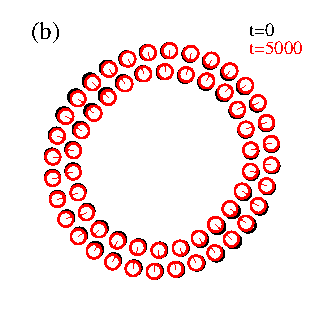
\includegraphics[height=2in]{relax2.eps}
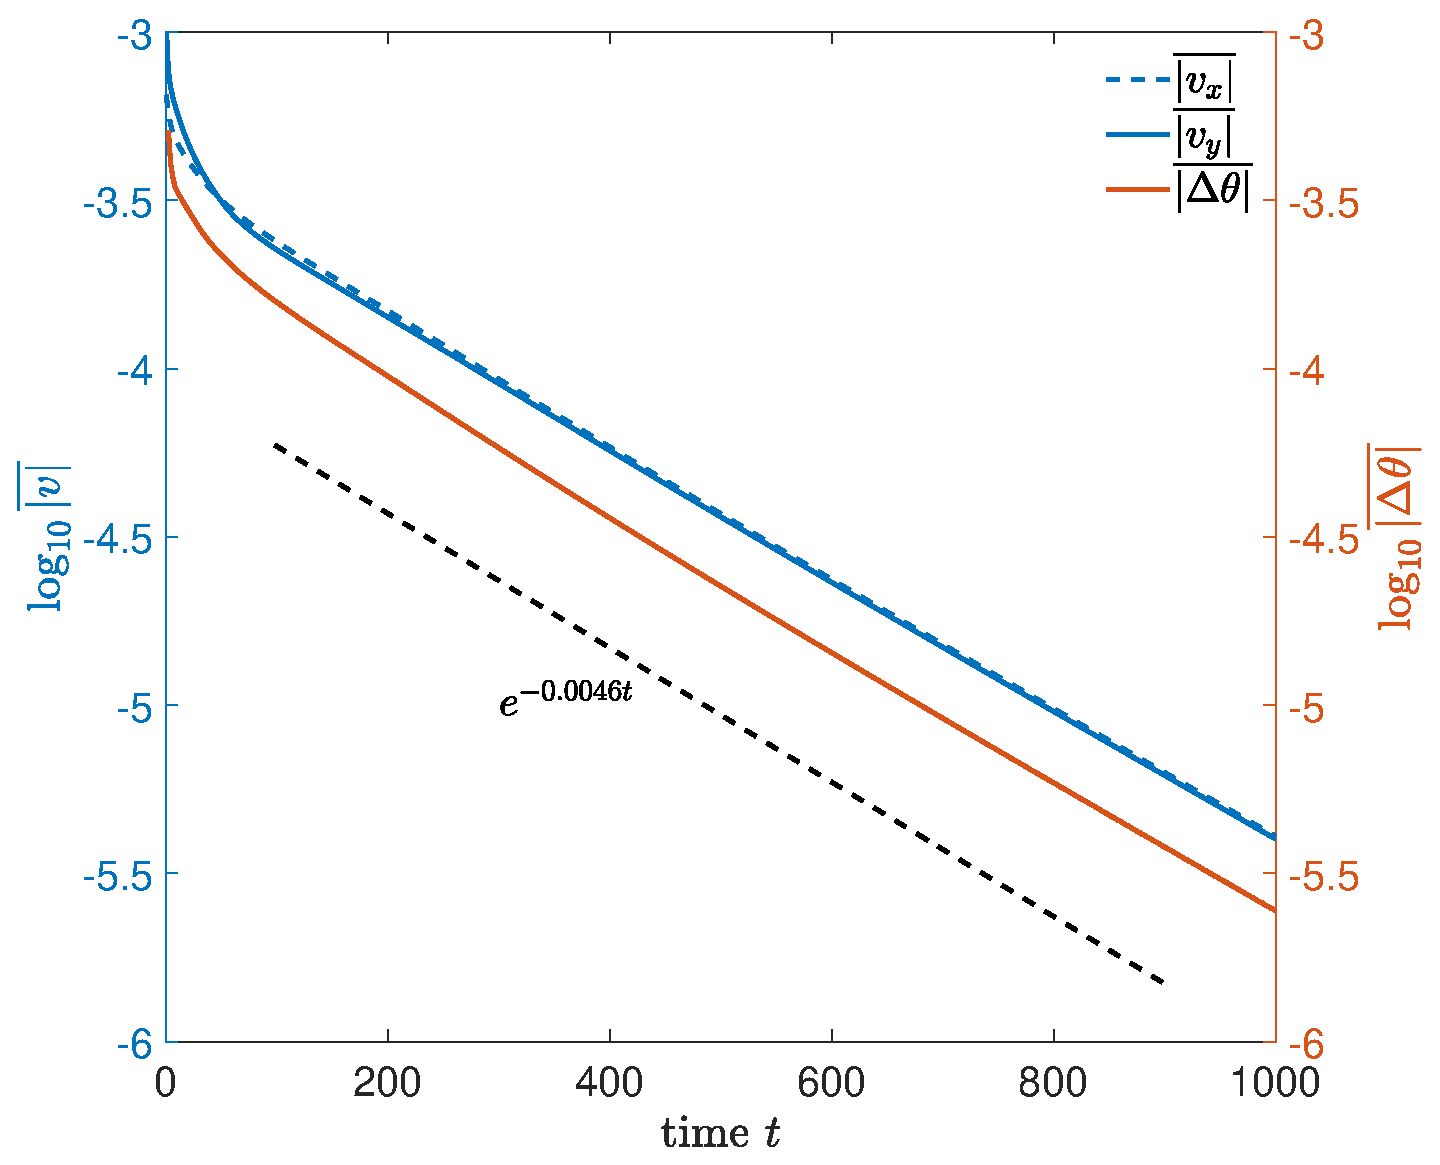
\includegraphics[height=2in]{relax.eps}\\
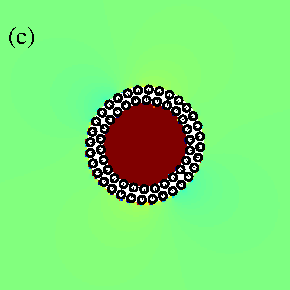
\includegraphics[height=2.in]{N58_0pres.pdf}
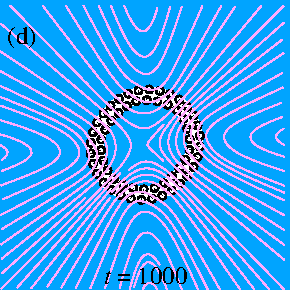
\includegraphics[height=2.in]{N58_5000pres.pdf}
%  \todo[inline]{Put pressure of each of the two configurations below
%  this.}
\caption{\label{figure2} A JP Vesicle relaxing under a quiescent flow.
  (a) The blue dashed and solid curves are mean magnitudes of the
  particle velocities in $x$ and $y$ directions, respectively. The red
  curve shows the decreasing trend of the mean magnitude of particle
  orientation change. The black dashed line shows the reference of how
  all magnitudes decay. (b) Bilayer configurations for $t=0$ (black) and
  $t=1000$ (red) with particle directors. (c)--(d) show the fluid
  pressure profiles for $t=0$ and $t=1000$ where the background curves
  indicate the streamlines. In panel (c), the pressure value in internal
  fluid is much higher than the pressure outside of the bilayer. After
  the JP vesicle relaxes, this immersed permeable bilayer approaches the
  steady state shown in panel (d).}
\end{figure}

In order to examine the hydrodynamics interactions of JP vesicles, it is
necessary to have a suitable, initial, JP equilibrium vesicle. This
ensures that the dynamics of the bilayer under a shear flow, for
example, reach consistent outcomes. For our target vesicle, we start
with $N=58$ JP arranged in two circular, apposing monolayers of about
$8$ length units. The directors of the outer monolayer point inward and
the directors of the inner monolayer point outward
(Figure~\ref{figure2}a).  The JP of this chosen configuration are
generally not in equilibrium.  Rather, the inter-particle distances and
orientations must make slight adjustments so that attraction and
repulsion balance.  Figure~\ref{figure2}(b) shows that the magnitudes of
the mean velocity components ${\bf v}=\{v_x,v_y\}$ and the variation
$\Delta \theta$ of the particle orientation decrease exponentially with
an approximation decaying rate $\sim0.005$. A local energy minimum and
the equilibrium configuration is therefore rapidly attained. The
equilibrium configuration in Figure~\ref{figure2}a is slightly
elliptical. The equilibrium eccentricity vanishes for larger $N_b$
(Figure~\ref{figure2}e).

\subsection{Permeability}
Figures~\ref{figure2}c and~\ref{figure2}d demonstrate that the initial, non-equilibrium configuration has a large internal fluid pressure
that vanishes as the configuration tends toward the equilibrium state.  
This suggests that the initial collection of JP is under tension and
this tension is relaxed as fluid is expelled through the inter-particle
spacing. To make a comparison with membrane continuum mechanics, lipid
bilayer membranes have a large area modulus $K_A$ of about $240$ pN
nm$^{-1}$ \cite{NAGLE} and changes in surface area give rise to a
membrane tension $\tilde \gamma = K_A(A/A_0 - 1)$ where $A$ is the
membrane surface area and $A_0$ is the reference surface area in the
non-tensed state. In the two-dimensional vesicles, the tension becomes
\begin{align}
\label{eq:stretch}
\tilde \gamma = K_A\left(\frac{L}{L_0} - 1 \right),
\end{align}
where $L$ and $L_0$ are the vesicle arc length and resting length,
respectively. A stretched, circular vesicles has a Laplace pressure 
\begin{align}
\label{eq:LaplacePressure}
\Delta p = \frac{\tilde \gamma}{R},
\end{align}
where $\Delta p$ is the difference in internal pressure to the pressure
at infinity and $R$ is the radius of the circular vesicle. The factor
$R^{-1}$ is the total curvature since the principle curvature in the
direction of the cylinder is zero.

\begin{figure}
\centering
  \todo[inline]{The left figure is shorter than the other 2}
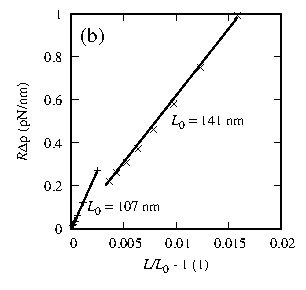
\includegraphics[width=0.32\textwidth]{PermPanelB.pdf}
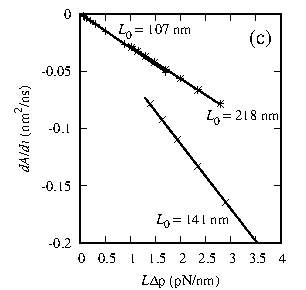
\includegraphics[width=0.32\textwidth]{PermPanelC.pdf}
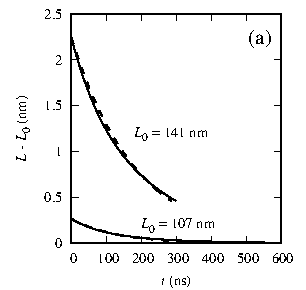
\includegraphics[width=0.32\textwidth]{PermPanelA.pdf}
  \caption{\label{figure:permeability} JP vesicles are suspended in a
  quiescent flow for relaxations where the reference arc lengths $L_0$
  are $107$ nm, $218$ nm, and $141$ nm with particle diameters $2.5$ nm,
  $2.5$ nm, and $1.25$ nm, respectively. (a) The arc length $L$
  decreases over time where the dashed curves represent the data and
  solid curves are linear fits; (b) A linear relationship between
  $R\Delta p$ and the relative difference $L/L_0-1$; (c) A linear
  relationship between aqueous flux $dA/dt$ and $L\Delta p$. For panels
  (b) and (c), the cross and asterisk symbols are numerical results and
  fitted by using solid lines.}
\end{figure}

The particles in our setup do not abut but rather have small gaps due to
repulsive forces.  The gaps allow for some fluid flux across the JP
bilayer.  In membrane mechanics, aqueous flux is quantified the equation
\begin{align}
  \label{eq:perm} 
  \frac{dA}{dt} = -P  L \Delta p,
\end{align}
where $P$ is a hydraulic permeability constant \cite{CHABANON,
qua-gan-you2021}.

The JP vesicle data is in complete agreement with the continuum
mechanical model~\eqref{eq:stretch}--\eqref{eq:perm}. In
Figure~\ref{figure:permeability}, we considered three configurations: a
configuration with 58 particles ($L_0 = 107$ nm, plus symbols); a
configuration with 119 particles ($L_0 = 218$ nm, asterisk symbols); and
finally a configuration with 117 particles but with diameter 1.25 nm
rather than the usual 2.5 nm ($L_0 = 141$ nm, times symbols). Here $A$
and $L$ refer to the area and length of the mid plane curve separating
the inner and outer monolayers. The values for $L_0$ are the asymptotic
values for $L$ in Figure~\ref{figure:permeability}c.

Figure~\ref{figure:permeability}a plots the data for the Laplace
pressure relationship \eqref{eq:LaplacePressure}. The pressure jump
$\Delta p$ is the pressure at the particle center minus the far-field
pressure (see Figures~\ref{figure2}c and~\ref{figure2}d), $R = L/2\pi$
is the vesicle radius, and the horizontal axis is the relative stretch.
The solid lines are linear fits, showing that for circular JP vesicles,
$R\Delta P$ is essentially proportional to the relative stretching
$L/L_0 - 1$. The proportionality constant is the same for the 58 and 119
particle cases where the diameters are the same, suggesting that the
stretching modulus $K_A$ of JP bilayers is independent of the number of
particles. The 117 particle case had diameters 1.25 nm and this data set
results in a smaller stretching modulus of $K_A = 102$~pN~nm$^{-1}$. The
interpretation is that changes to particle size, while keeping $\rho$,
$M$, and $\rho_0$ fixed, lead to different physical properties.

Furthermore, Figure~\ref{figure:permeability}b and shows that $L\Delta
P$ is proportional to $\frac{dA}{dt}$ in accord with \eqref{eq:perm}.
The slopes of the linear fits give the hydraulic permeability
coefficient $P$. The data provide $P = 0.0296$ nm$^3$ ns$^{-1}$
pN$^{-1}$ and $P = 0.0283$ nm$^3$ ns$^{-1}$ pN$^{-1}$ for the 58 and 119
particle cases, respectively. These values suggest that the JP bilayer
permeability is independent of particle number, as was the case for the
stretching modulus. The permeability for the 117 particle number is
0.0566 nm$^3$~ns$^{-1}$~pN$^{-1}$. The increase in the permeability is
caused by the hydrophobic attraction vanishing with particle size,
leading to larger gaps between the particles for the same repulsion. The
hydraulic permeability we calculate, however, is not in agreement with
experimentally derived values and is larger by a few orders of
magnitude. This discrepancy is perhaps due to inter-particle distance of
the JP being relatively large to the inter-molecular spacing of lipids
in real bilayers. In future studies, we can test this hypothesis be
changing the repulsion strength and length for example. 

Since the vesicles in Figure~\ref{figure2}a are nearly circular, we can
combine~\eqref{eq:stretch},~\eqref{eq:LaplacePressure},
and~\eqref{eq:perm}, to derive
\begin{align}
\label{eq:perm_solution}
L_0(L-L(0)) + L_0^2 \ln\left|\frac{L-L_0}{L(0)-L_0}\right| = -4\pi^2 P K_A t.
\end{align}
The theoretical time courses for \eqref{eq:perm_solution} are in good
quantitative agreement with the JP data for
(Figure~\ref{figure:permeability}c).




%\subsection{Jeffery Orbit}
%We use Jeffery orbits to numerically validate our solver for the mobility-problem.  
%The background flow is a shear flow $\uu_{\infty}(\xx) = \dot\gamma  \xx \cdot \mathbf{e}_2 \mathbf{e}_1$ with shear rate $\dot\gamma$
%and orthogonal unit vectors $\mathbf{e}_1$ and $\mathbf{e}_2$. 
%A single elliptical particle is suspended in the fluid with center at the origin.
%The Jeffrey orbit  
%\begin{equation}
%\label{eq:jeff}
%\Theta(t) = \tan^{-1}\left(\frac{a}{b}\tan \left(\frac{ab \dot\gamma t}{a^2+b^2}\right)\right)
%\end{equation}
%gives the angle between the major axis and $\mathbf{e}_2$
%where $a$, $b$ are the semi-major and semi-minor axes. 
%We are assuming $\Theta(0) = 0$.
%Figure~\ref{figure1} shows that the angles coming from the integral equation method \eqref{eq:SKIE}-\eqref{eq:mobility2}
%are in complete agreement with the theoretical time course \eqref{eq:jeff}.  Hydrophobic attraction and repulsion are zero for a single particle. 
%
%
%\begin{figure}
%\centering
%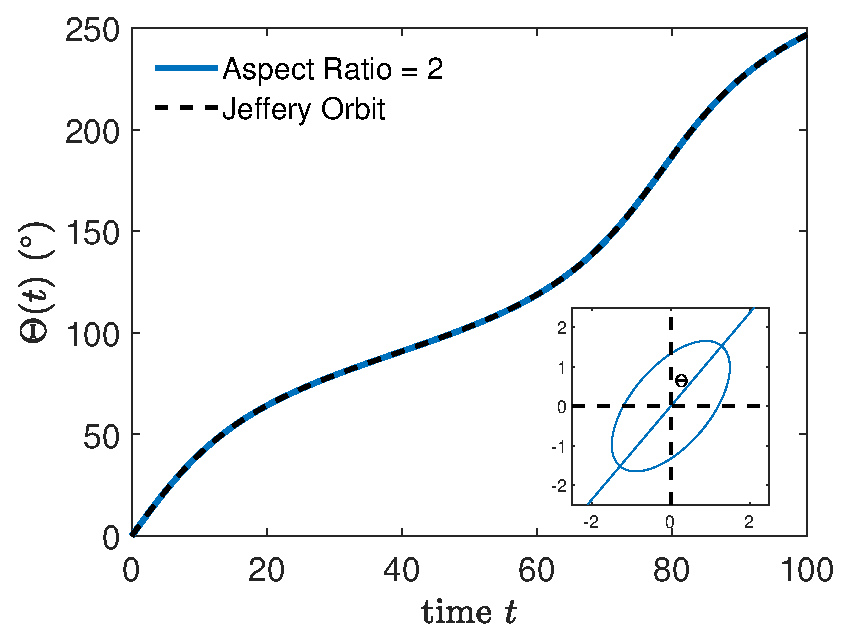
\includegraphics[width=0.4\textwidth]{JefferyOrbit2.eps}
%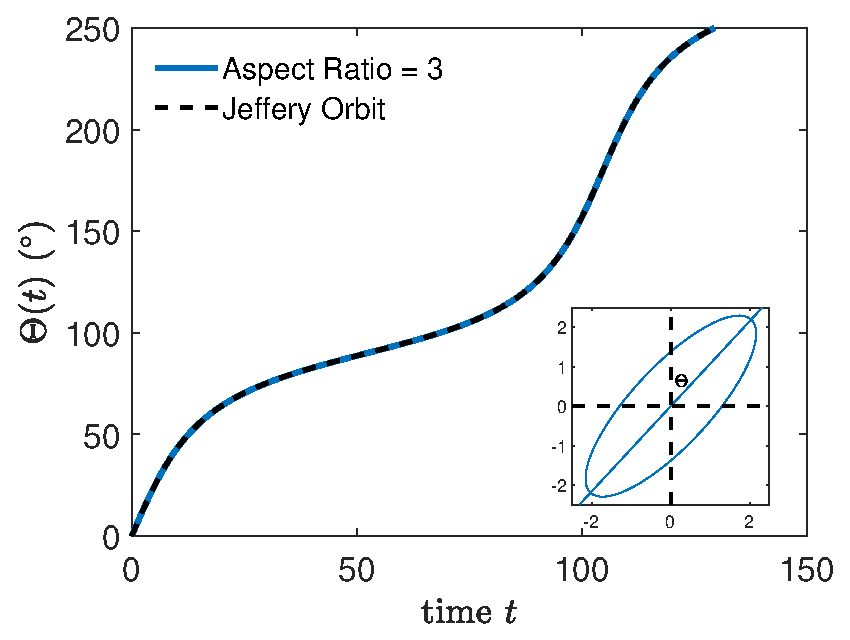
\includegraphics[width=0.4\textwidth]{JefferyOrbit3.eps}
%  \caption{The figure compares the theoretical Jeffery orbit for $\Theta(t)$ and the result from the integral equation method. 
%    The insets show the simulation setup. The shear rate is $\dot\gamma=0.1$.}
%    \label{figure1}
%\end{figure}

%%%%%%%%%%%%%%%%%%%%%%%%%%%%%%%%%%%%%%%%%%%%%%%%%%%%%%%%%%%%%%%%%%%%%%%



%%%%%%%%%%%%%%%%%%%%%%%%%%%%%%%%%%%%%%%%%%%%%%%%%%%%%%%%%%%%%%%%%%%%%%%

%\todo[inline]{Introduce dimensionless shear rate here (and check the numbers)}




%For the $N$-body Janus-vesicle, we denote a constant initial radius $R_0=\sqrt{A_0/4\pi}$ with initial area $A_0$

%referred from~\cite{Finken08} and~\cite{Shaqfeh11},
%\begin{align}
%  \chi = \dot\gamma \frac{\mu R_0^3}{\kappa},
%\end{align}
%%
%where $\dot\gamma$ the dimensional shear rate, and $\mu$ the fluid viscosity.


%%%%%%%%%%%%%%%%%%%%%%%%%%%%%%%%%%%%%%%%%%%%%%%%%%%%%%%%%%%%%%%%%%%%%%%
\subsection{Tank-Treading Vesicles}

%%%%%%%%%%%%%%%%%%%%%%%%%%%%%%%%%%%%%%%%%%%%%%%%%%%%%%%%%%%%%%%%%%%%%%%
\subsubsection{Vesicle in a Shear Flow}
\label{sec:ves_in_shear}
Our hydrodynamic simulation studies begin by studying the dynamics of a single JP vesicle suspended in
the shear flow
\begin{align}
  \uu_{\infty}(\xx) = \dot\gamma (\xx \cdot \mathbf{e}_y) \mathbf{e}_x,
\end{align}
with shear rate $\dot\gamma$, and orthogonal unit vectors $\mathbf{e}_x$
and $\mathbf{e}_y$ for the horizontal and vertical directions,
respectively. It is well known that a vesicle has tank-treading behavior
when there is no viscosity contrast between the fluids inside and
outside of the vesicle.
%Within the framework of the simulation setup,
%the proposed model provides a feature that the fluid viscosity is
%constant over the computational domain and it is capable of performing
%these simulations.

The centroid of the pre-relaxed $58$-body Janus vesicle is initially
placed at the origin and the shear flow with a shear rate $\chi$ is
applied. Figure~\ref{figure3} shows snapshots of the JP vesicle in the
shear flow with a shear rate $\chi=0.0025$. Panels (a) and (b) show the
initial shape obtained from the relaxation run and the deformed
configurations of the JP vesicle at time $t=4000$ are in panels (c) and
(d). The background color in panels (a) and (c) is the strength of the
action of the hydrophobic attraction. Red corresponds to a strong action
while blue is a weak action. The hydrophobic layer clearly has the
strongest action. To demonstrate the tank-treading behavior of the
vesicle, panels (b) and (d) provide the streamlines of the fluid
velocity around the JP vesicle. In panel (d), we can clearly observe the
clockwise tank-treading motion.


\begin{figure}
\centering
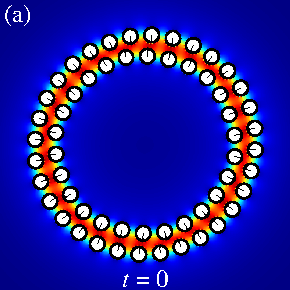
\includegraphics[width=0.3\textwidth]{N58_0.pdf}
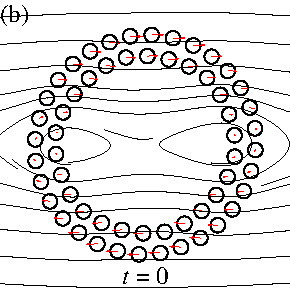
\includegraphics[width=0.3\textwidth]{N58_vel_0.pdf}\\
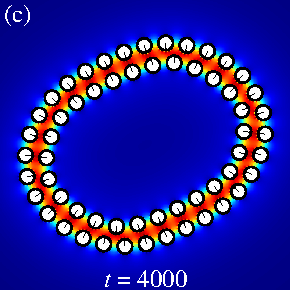
\includegraphics[width=0.3\textwidth]{N58_20000.pdf}
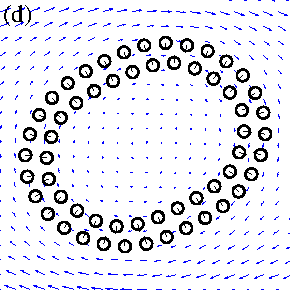
\includegraphics[width=0.3\textwidth]{N58_vel_20000.pdf}
  \caption{\label{figure3} A JP vesicle suspended in a shear flow with
  shear rate $\chi=0.0025$. (a) The initial configuration of a 58-body
  JP vesicle where the black arrows point in the direction of the
  hydrophobic side of the JP. (b) The particle velocities and
  streamlines of the configuration in (a). The streamlines are plotted
  in the background as solid curves and the red arrows represent the
  particle velocities. (c) The deformed tank-treading JP vesicle at
  $t=4000$. (d) The particle velocities and streamlines of the
  configuration in (c). The background colors in panels (a) and (c)
  represent the strength of the hydrophobic attraction potential. The
  blue regions have the weakest action and the red regions in the
  bilayer have the strongest action.}
\end{figure}
%

To extract additional physical properties of the proposed model, we
compute the total length, reduced area, and excess length of the bilayer
structure. The enclosed area and the total length of the structure are
calculated from the midplane. The reduced area is $A^* = 4\pi A/L^2$
where $A$ is the area, and $L$ is the total length of the JP vesicle,
and the excess length is $\Delta=L/\sqrt{A^*/\pi}-2\pi$.
Figure~\ref{figure4} shows these quantities for a JP vesicle suspended
in a shear flow with shear rates $\chi=\{0.002,0.0025,0.003,0.0035\}$.
Since the starting configuration is nearly circular, the reduced area
decreases from an initial value close to $1$. The smooth curves in panel
(a) are best fits of the exponential model $A^* = a_0 + b_0 \exp(-kt)$.
Panel (b) shows that the decay rate $k$ is independent of the shear rate
for sufficiently large shear rates, and the terminal reduced areas of
each case are shown in the inset. We see that lower shear rates generate
a higher final reduced area. In particular, we observe that the reduce
area converges relatively early when the shear rate is lower than
$\chi=0.003$. 
%and has a faster convergence than the high shear rate cases.
Panel (c) shows that the total arc length remains constant for all time
with all four shear rates. Combining the behavior of the reduced area
and the total arc length, the excess length must increase in time and be
larger for higher shear rates as observed in panel (d). In all these
results, there are oscillations that can be explained by the granularity
of the JP vesicle which results in a midplane that is non-smooth.
%Overall the total lengths of the bilayer have the same converging value
%in all test shear rates.

\begin{figure}
\begin{center}
\hspace{-0.6cm}
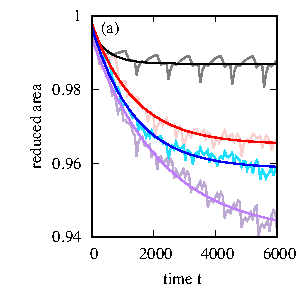
\includegraphics[height=2in]{ReducedArea.pdf}
\hspace{0.6cm}
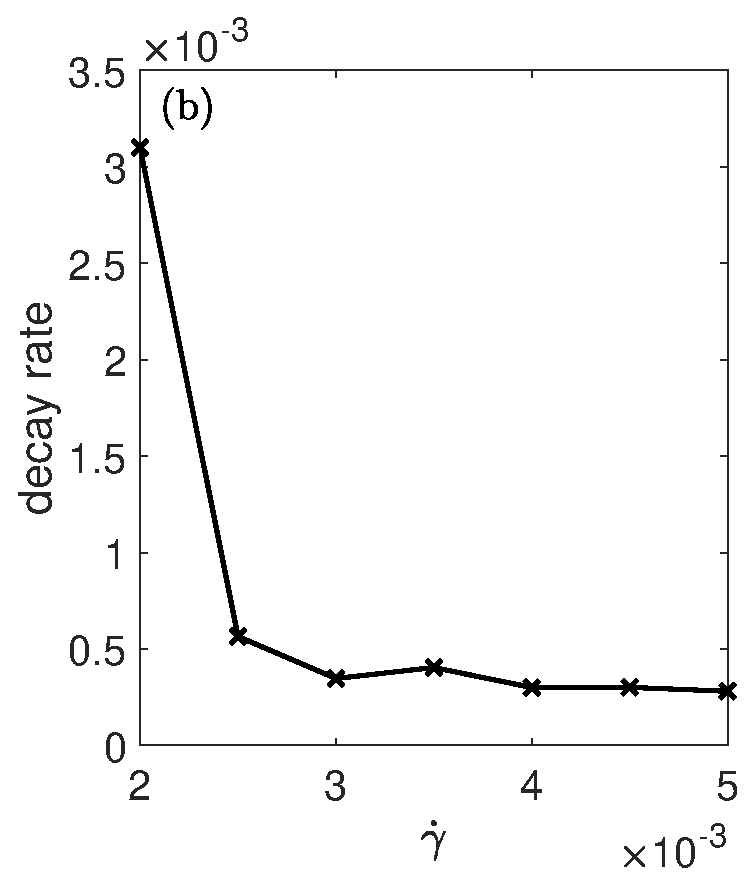
\includegraphics[height=2in]{DecayRate.eps}\\
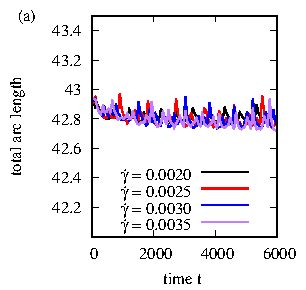
\includegraphics[height=2in]{ArcLength.pdf}
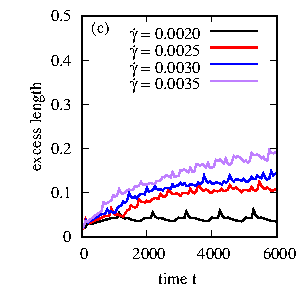
\includegraphics[height=2in]{ExcLength.pdf}
\end{center} 
  \caption{\label{figure4} (a) The reduced area transitioning over time
  for four different shear rates. The smooth curves are a best-fit
  exponential curve. (b) The decay rate $k$, using the exponential fit
  to the data in panel (a), for a number of shear rates. The inset shows
  the terminal reduced areas. (c) The total arc lengths of the midplanes
  over time for four shear rates. (d) The excess length of the
  midplanes. For all panels, a set of shear rates
  $\chi=\{0.002,0.0025,0.003,0.0035\}$ is used in simulations. The
  legend in panel (d) applies to both panels (a) and (c).}
\end{figure}


%%%%%%%%%%%%%%%%%%%%%%%%%%%%%%%%%%%%%%%%%%%%%%%%%%%%%%%%%%%%%%%%%%%%%%%
\subsubsection{Intermonolayer Friction}
The granulated JP vesicle allows us to consider inter-monolayer slip
between the two leaflets. When the shear rate is sufficiently large,
take $\chi = 0.005$ as an example, Figure~\ref{figure5} shows slip
between a pair of particles over time. The pair we consider are colored
in blue and yellow. In this series of tests, we compute the mean
particle position and mean angle $\theta(t)$ between the particle
relative positions with respect to the vesicle center. It is clear that
the outer leaflet has larger tangential velocity than the inner leaflet
since $\theta(t)$ increases. This inter-leaflet sliding phenomenon is
consistent with what has been seen in articles in molecular dynamics
simulations.
\todo[inline]{Need a reference here}


\begin{figure}
\begin{center}
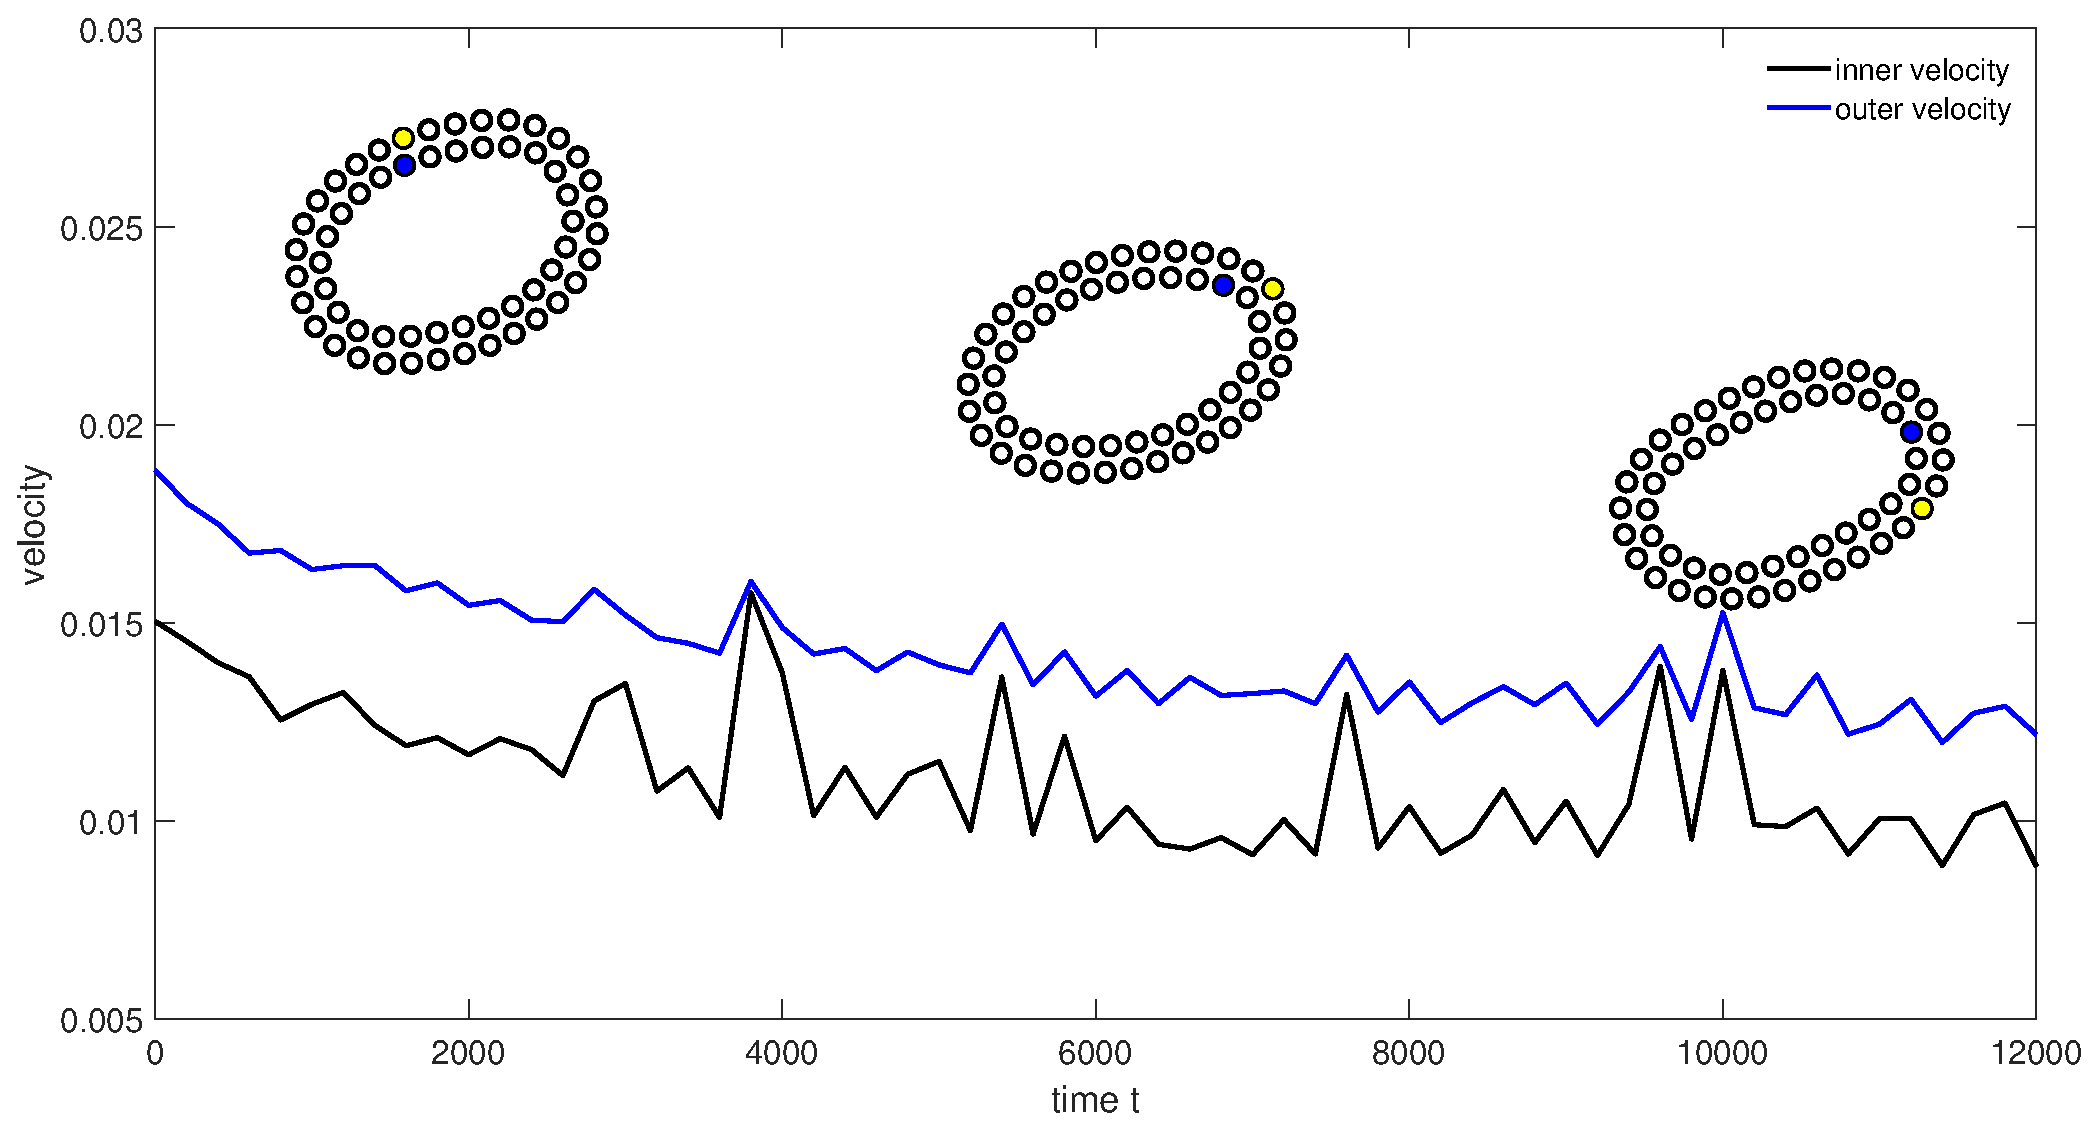
\includegraphics[width=0.5\textwidth]{Slip.eps}
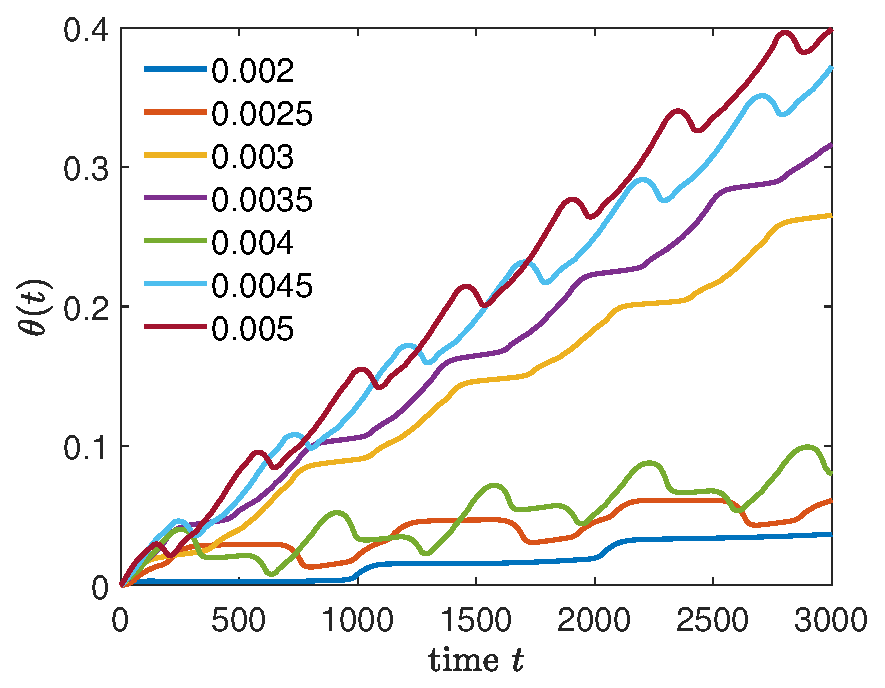
\includegraphics[width=0.4\textwidth]{Slip2.eps}
\end{center} 
  \caption{\label{figure5} The schematic of the intermonolayer slip over
  time. Taking a shear rate $\chi=0.005$ as an example, we denote the
  mean angle between each particle pair $\theta(t)$ where the angle is
  calculated from the relative position of the particles with respect to
  the JP vesicle's center of mass. The configuration plots have two
  fixed particles marked in yellow and blue and labeled with the
  corresponding time $t=2000$ and $t=9000$. The midplane curve is
  denoted as $\Sigma_M$. We see that the intermonolayer slip is largest
  for large shear rates.}
\end{figure}

To calculate the inter-monolayer friction coefficient for the apposing
JP leaflets, we let
\begin{align}
  b = \frac{\langle F\rangle}{\langle L \rangle \langle U\rangle},
\end{align}
%
where 
\begin{align}
  \langle F\rangle = \left\langle \int_{\mathcal{C}_M} 
    \jump{\ttau \cdot \sigma \cdot \nnu} \,\dif s \right\rangle
\end{align}
is the time-averaged, tangential force along the midplane curve
$\mathcal{C}_m$. The parameters $\langle L\rangle$ and $\langle
U\rangle$ are the time-averaged midplane curve length and intermonolayer
slip velocity, respectively.

We calculate $\langle F\rangle$ by first evaluating the smooth
tangential force along curves a positive distance inside and outside
$\mathcal{C}_m$ respectively, and then interpolating at zero distance to
give a force jump. We have made a slight abuse of language: due to the
problem being two-dimensional, the integral $\langle F\rangle$ is
actually a force density per length which when divided by length gives
the requisite force per area. 
%which when divided by length 

Table~\ref{table1} provides dimensional friction coefficients $b$ for
several shear rates and the results are in quantitative agreement with
values previously reported in the literature (\cite{sch-vla-mik2010}
and~\cite{denOtter2007}). The coefficients generally lie within the
range 0.2 to 0.3 pN$\cdot$ns nm$^{-3}$ but there are some outliers.
These outliers ($\dot\gamma = 0.0041$ ns$^{-1}$ and $\dot\gamma =
0.0066$ ns$^{-1}$) correspond to slip velocities that are too low
relative to the shear rate (see the green and red curve in
Figure~\ref{figure5}(c)). The JP vesicle consists of only 58 particles
and so it is not surprising that discrete effects produce outliers.

%\todo[inline]{If $B$ is the numerically calculated friction coefficient,
%then $b = B/2.5^3$ pN ns nm$^{-3}$ gives the dimensional value.
%
%If $P$ is the numerically calculated pressure, then $p = P/2.5$ pN
%nm$^{-2}$ is the dimensional pressure.} 

\begin{table}
\caption{Friction Coefficients}
\centering
\begin{tabular}{c c c c c c c c }
 $\chi$ & 0.0020   &  0.0025 &  0.0030 &  0.0035 &  0.0040 & 0.0045 & 0.0050  \\
\hline                    
$\dot\gamma$ (ns$^{-1}$)        & 0.0033 & 0.0041 & 0.0049 & 0.0057 & 0.0066 & 0.0074 & 0.0082\\
%$F_{f}$ (pN nm$^{-1}$)           & 1.84 & 4.90 & 11.36 & 8.16 & 6.14 &  17.69 &  24.33 \\[1ex]
%$\dot\theta$ (nm ns$^{-1}$)           & $6.84\times10^{-5}$ & $1.31\times10^{-4}$ & $3.46\times10^{-4}$ & $2.32\times10^{-4}$ & $1.81\times10^{-4}$ & $4.91\times10^{-4}$ & $5.83\times10^{-4}$\\ [1ex]
$b$ (pN$\cdot$ns nm$^{-3}$)    & 0.22 & 0.87  & 0.22 &0.21 & 1.29 & 0.31 & 0.30\\ 
\hline    
\end{tabular} 
\label{table1}
\end{table}


%%%%%%%%%%%%%%%%%%%%%%%%%%%%%%%%%%%%%%%%%%%%%%%%%%%%%%%%%%%%%%%%%%%%%%%
\subsubsection{Vesicle in a Parabolic Flow}
Another interesting flow to consider is the parabolic flow
\begin{align}
  \uu_\infty = v_{max}\left[ 1 - \left( 
    \frac{\xx \cdot \mathbf{e}_y}{wR_0}\right)^2
    \right]\mathbf{e}_x,
\end{align}
%
where $v_{max}$ is the flow strength and $w$ determines the shape of the
flow. $R_0$ is defined as the radius of the JP vesicle at $t=0$. The
behavior of a vesicle in this unbounded non-linear flow includes
vertical migration, and depending on the flow rate and reduced area, the
steady-state shape can be either a symmetric parachute or an asymmetric
slipper (\cite{Kaoui09, cou-kao-pod-mis2008, dan-vla-mis2009}).

%Besides the tests of a JP vesicle in a shear flow, an interesting
%test can also use the proposed model and the setup. Consider a
%symmetric parabolic flow about the $x$-axis,~\cite{Kaoui09} studied
%shapes of the red blood cell immersed in a parabolic flow using a
%continuum model. With a similar setup, the background flow for this set
%of simulations is given by

Figure~\ref{figure6} shows three configurations for one specific case
where the centroid of the JP vesicle is initially placed slightly
above the $x$-axis. The parameters are $v_{max} = 8.0$, $w=10$, and
$R_0=8$. The red curves are the midplanes and a particle pair is marked
in color. We observe that the deformed JP vesicle has a
counterclockwise movement and the shape of the vesicle approaches an
asymmetric slipper shape. Moreover, we observe inter-monolayer slip
between the two leaflets. For this test, the reduced area for this
configuration is approximately $0.9$ which matches the previous
numerical tests in~\cite{Kaoui09} where a slipper-like shape occurs when
the flow velocity is weak and the reduced area is large. A schematic of
the setup is shown in Figure~\ref{figure7} where the blue horizontal
line represents the mean $y$-position of all particles. The inset of
Figure~\ref{figure7} shows the trajectory of the mean position in the
$y$-direction that decreases towards $y=1$ for a period of time and then
starts to oscillate due to the granularity of the JP vesicle. 

\begin{figure}
\centering
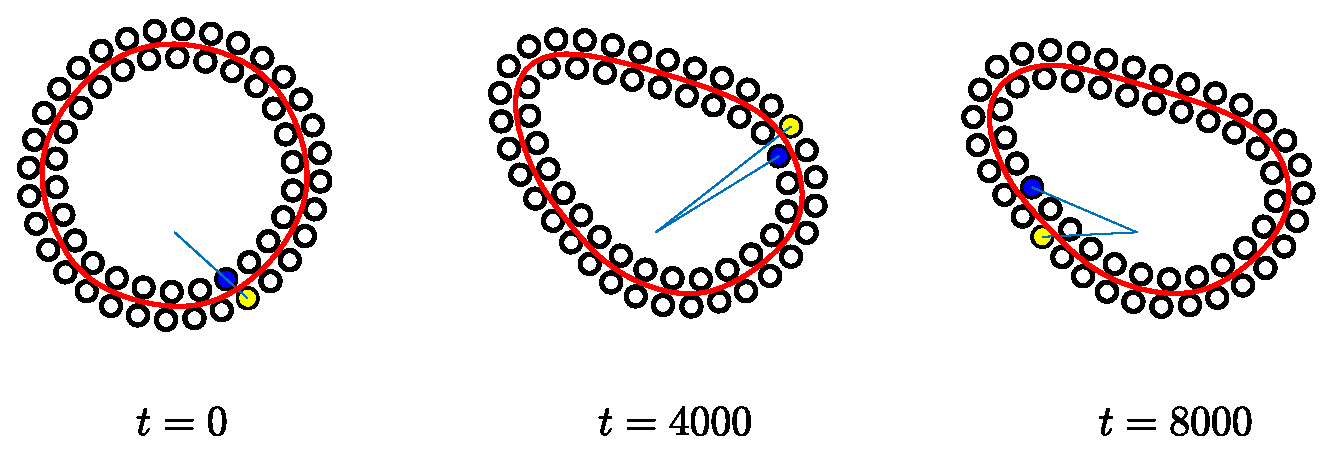
\includegraphics[width=0.8\textwidth]{slipper.eps}
  \caption{\label{figure6} A JP vesicle suspended in a parabolic flow
  where the strength of the flow is $v_{max}=32.8$~nm ns$^{-1}$, $R_0 =
  20$~nm, and the control parameter is $w=25$~nm. The configuration is
  the state when $t=\{0, 4000, 8000\}$. The red curves are the
  midplanes. Inter-monolayer slip is observed by comparing the relative
  locations of the blue and yellow particles.}
\end{figure}


\begin{figure}
\centering
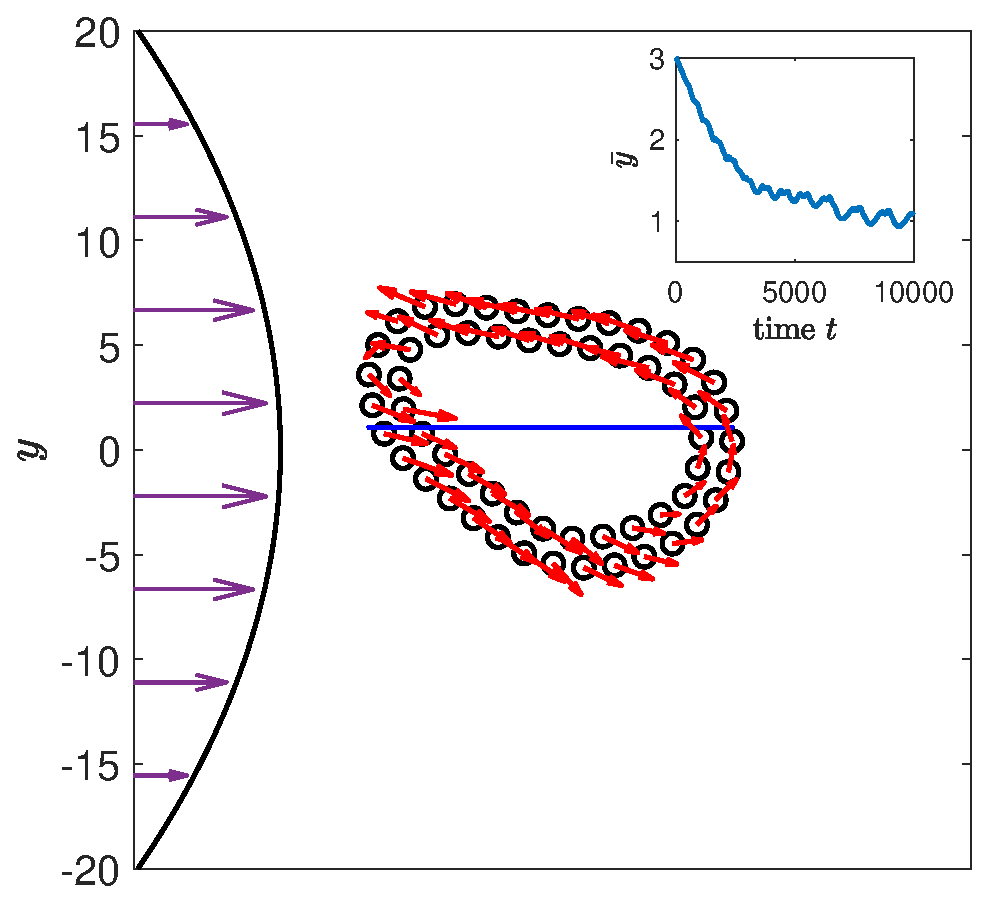
\includegraphics[height=2in]{parabolic.eps}
  \caption{\label{figure7} The schematic of a JP vesicle suspended in a
  parabolic flow where the strength of the flow is
  $v_{max}=32.8$~nm~ns$^{-1}$, $R_0 = 20$~nm, and the control parameter
  is $w=25$~nm. The configuration occurs when $t=10000$. The inset plots
  the trajectory of mean $y$-position over time.}
\end{figure}


%%%%%%%%%%%%%%%%%%%%%%%%%%%%%%%%%%%%%%%%%%%%%%%%%%%%%%%%%%%%%%%%%%%%%%%
\subsubsection{Membrane Ruptures}

A pore formation or a complete membrane rupture can occur at large shear
rates. Figure~\ref{figure8} demonstrates how a vesicle can rupture when
suspended in a shear flow with shear rate $\chi=0.1$. The streamlines
are included in these plots. An interesting phenomenon occurs in panels
(c) and (d) where two separated bilayers move along the background shear
flow symmetrically. Consequently, a periodic motion for bilayers may
occur at certain shear rates. One can expect that these two layers will
diverge from one another for much higher shear rates.

\begin{figure}
\centering
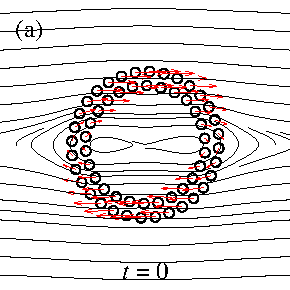
\includegraphics[height=2in]{N58_rupt_0.pdf}
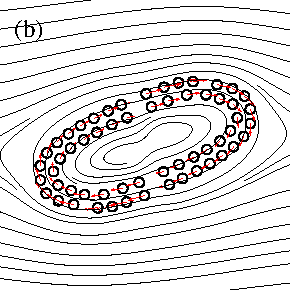
\includegraphics[height=2in]{N58_rupt_200.pdf}
\\
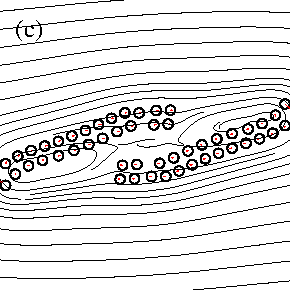
\includegraphics[height=2in]{N58_rupt_400.pdf}
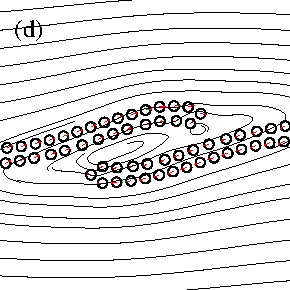
\includegraphics[height=2in]{N58_rupt_600.pdf}
  \caption{\label{figure8} Membrane rupture occurs when the shear rate
  exceeds a threshold. Here the shear rate is $\chi = 0.1$. Starting
  with a circular shape (panel (a)), the vesicle is stretched by the
  background flow and multiple pores form (panel (b)). Panels (c)--(d)
  show the later states during the simulation. Streamlines are included
  in each panel.}
\end{figure}


%%%%%%%%%%%%%%%%%%%%%%%%%%%%%%%%%%%%%%%%%%%%%%%%%%%%%%%%%%%%%%%%%%%%%%%
\subsection{Two Vesicles in a Linear Flow}

\begin{figure}
\begin{center}
  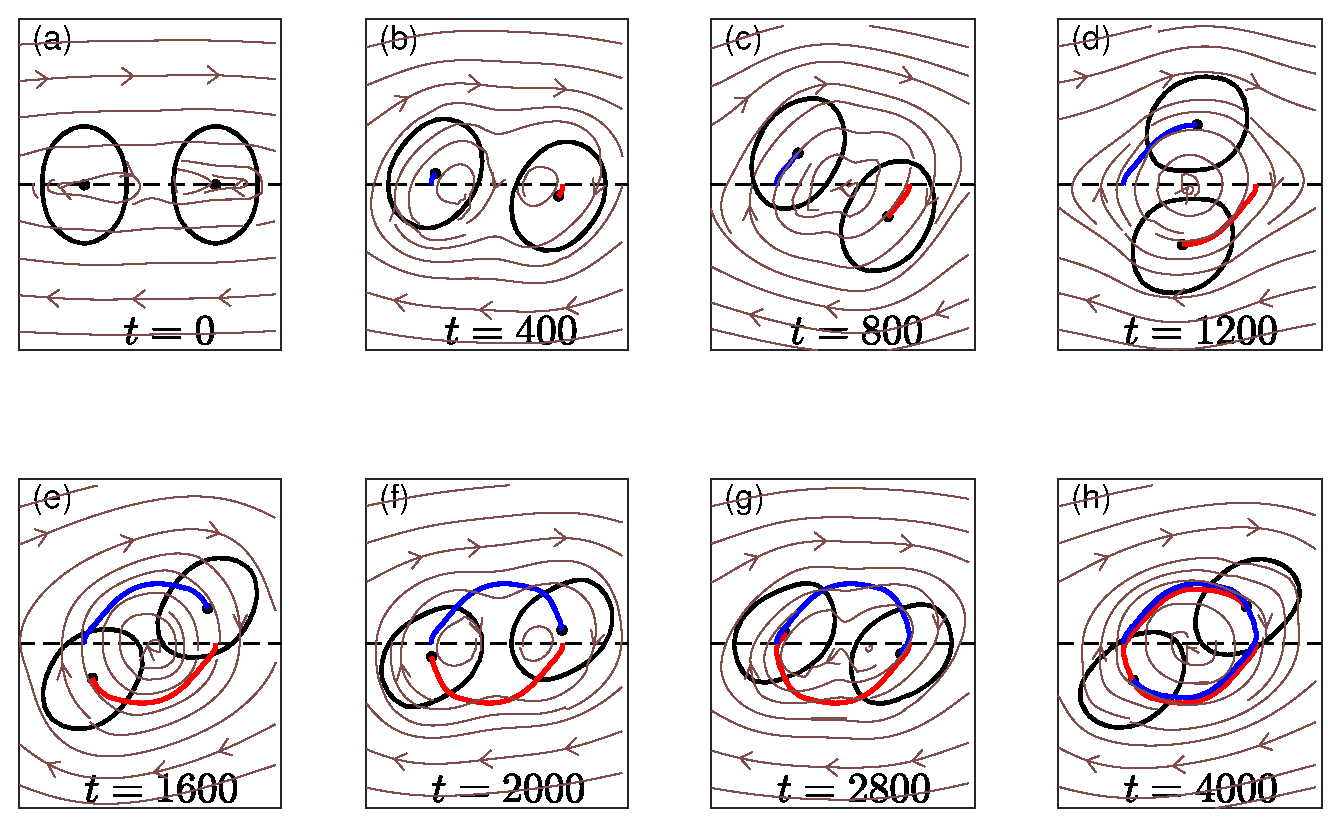
\includegraphics[width=0.9\textwidth]{ShearTraj.eps}
\end{center} 
  \caption{\label{figure9} The shape and trajectories of two
  JP vesicles suspended in a shear flow. The moving paths of the two
  centroids are plotted in blue and red. The centroids are initially
  located on the $x$-axis. For simulation time, $t = {0, 400,800,1200}$
  for (a)--(d) and $t = {1600, 2400, 3200, 4000}$ for (e)--(h).}
\end{figure}

\begin{figure}
\centering
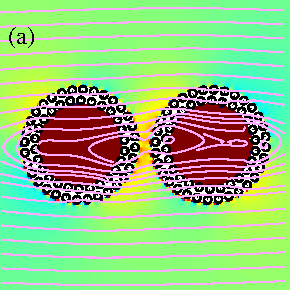
\includegraphics[height=2in]{N116_shear_0.pdf}
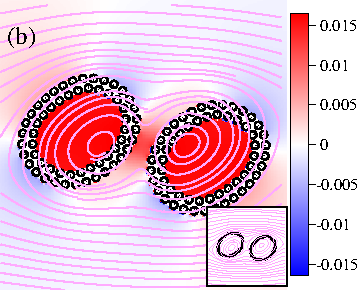
\includegraphics[height=2in]{N116_shear_2500.pdf}\\
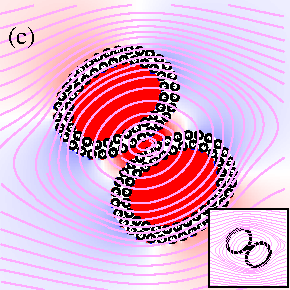
\includegraphics[height=2in]{N116_shear_5000.pdf}
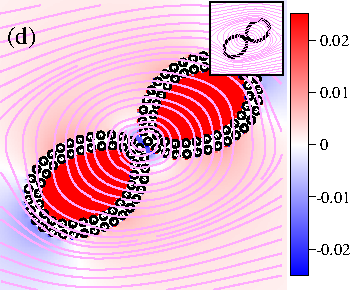
\includegraphics[height=2in]{N116_shear_7500.pdf}
  \caption{\label{figure10} Two JP vesicles suspended in a shear flow
  where the dimensioneless shear rate is $\chi=0.005$. The initial
  configuration is shown in panel (a). The background color is the fluid
  pressure. The color bar is identical for all panels. Streamlines are
  plotted in purple. The insets of all panels are generated from
  simulations of a continuum model of the vesicles and the streamlines
  agree between the two models.}
\end{figure}

%%%%%%%%%%%%%%%%%%%%%%%%%%%%%%%%%%%%%%%%%%%%%%%%%%%%%%%%%%%%%%%%%%%%%%%
\subsubsection{Shear Flow}

Figure~\ref{figure9} shows the simulation of two JP vesicles suspended
in a shear flow with shear rate $\chi=0.005$. We duplicate the
pre-relaxed $58$-body JP vesicle from previous sections to construct the
initial configuration shown in Figure~\ref{figure9}(a). The two centers
of mass are at $(-10,0)$ and $(10,0)$. In all panels, the blue and red
curves show the trajectory of the two JP vesicle centroids. They have
nearly completed a full period by $t=4000$. We also observe an adhesive
effect between the two JP vesicles that is set up by the hydrophobic
interactions and repulsive force. Similar dynamics have been observed
between a pair of adhering vesicles in a shear flow
(\cite{qua-vee-you2019, abb-far-ezz-ben-mis2021}). This adhesive
behavior is absent when two JP vesicles are well-separated.

Snapshots of the fluid pressure are in Figure~\ref{figure10}. Since the
initial JP vesicles are pre-relaxed, there is initially no pressure jump
between the internal and external fluids (panel (a)). Panels (b)--(d)
show the configurations when $t = \{500,1000,1500\}$, and the
streamlines are plotted in the background for all panels. We include the
numerical results from a continuum model in all insets and these
comparisons give a qualitative agreement between two models.

\begin{figure}
\begin{center}
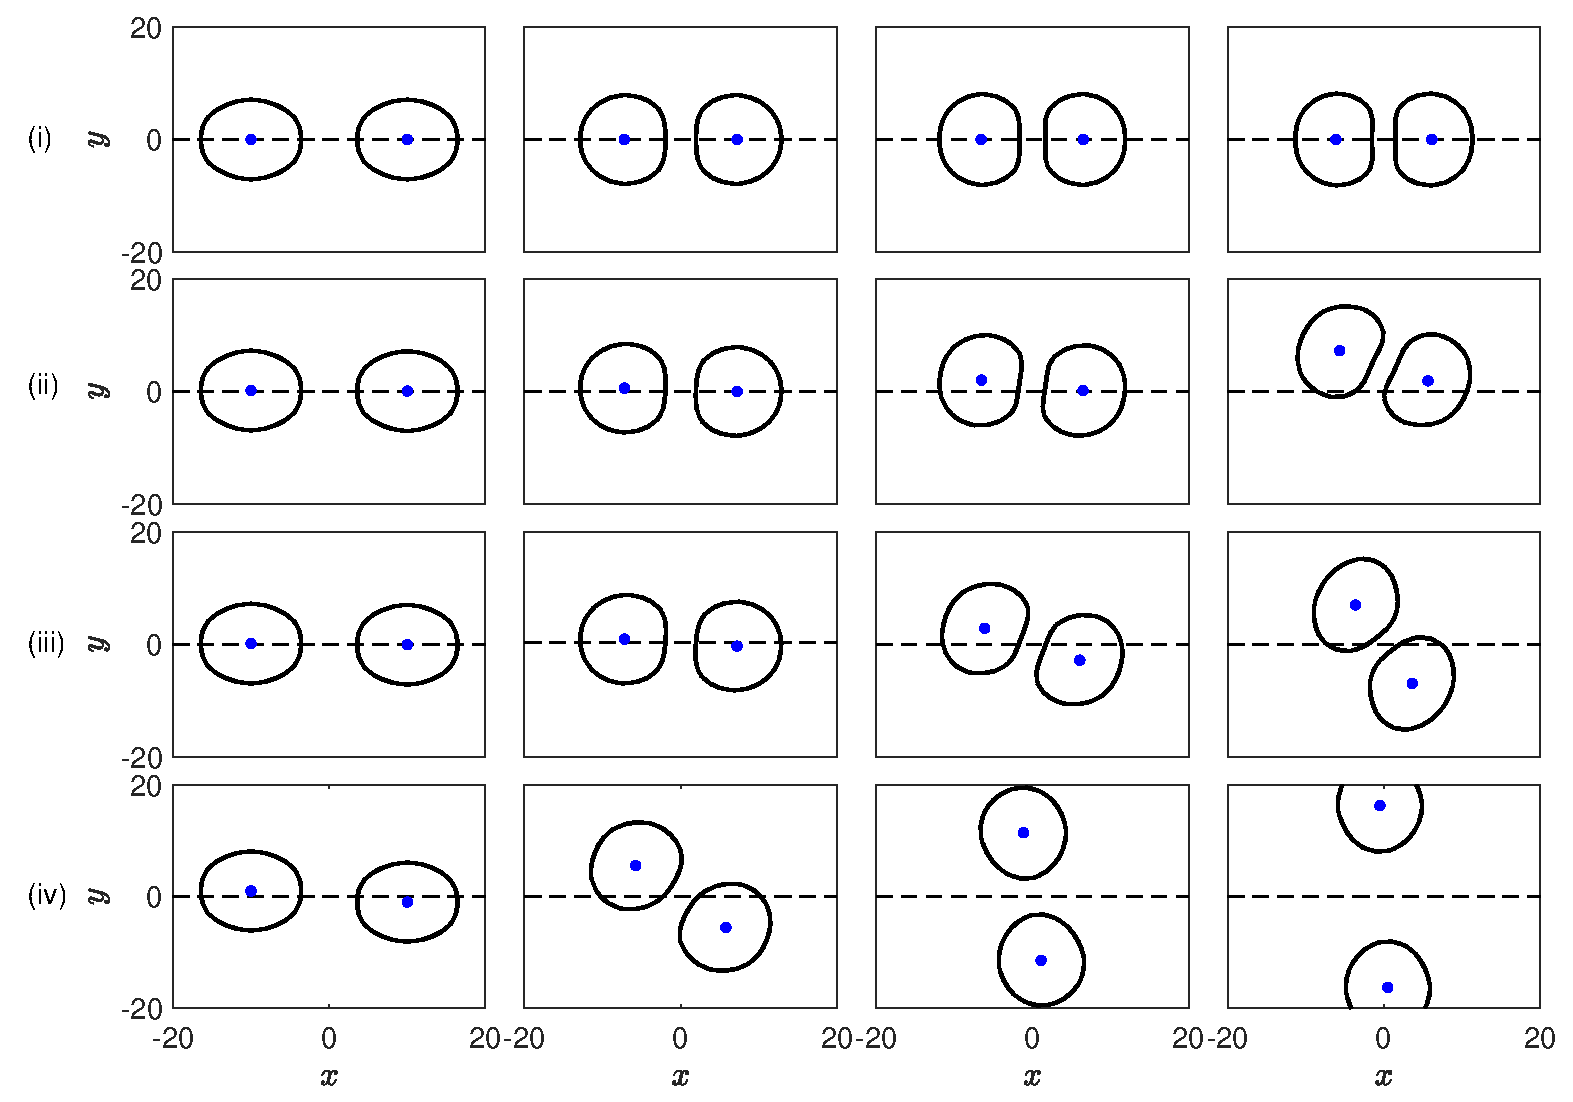
\includegraphics[width=0.9\textwidth]{ExtTraj.eps}
\end{center} 
  \caption{\label{figure11} Two JP vesicles suspended in
  an extensional flow. The moving paths of the two centroids are plotted
  in blue in red. Each row corresponds to a different initial placement
  of the JP vesicles. The flow rate is $\chi = 0.005$ in all cases.
  (i) Both JP vesicle centroids are on the $x$-axis. (ii) The
  centroid of the left JP vesicle is $0.1$ units above the $x$-axis
  and the right JP vesicle is on the $x$-axis. (iii) The centroid of
  the left JP vesicle is $0.1$ units above the $x$-axis and the right
  JP vesicle is $0.1$ units below the $x$-axis. (iv) The centroid of
  the left JP vesicle is $0.5$ units above the $x$-axis and the
  centroid of the right JP vesicle is $0.5$ units below the $x$-axis.
  Figure~\ref{figure12} presents the numerical results from the case
  (iii).}
\end{figure}


\begin{figure}
\centering
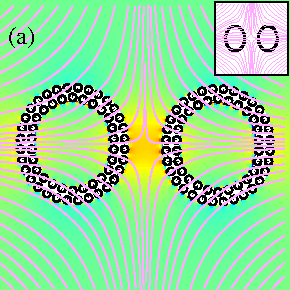
\includegraphics[height=2in]{N116_ext_0.pdf}
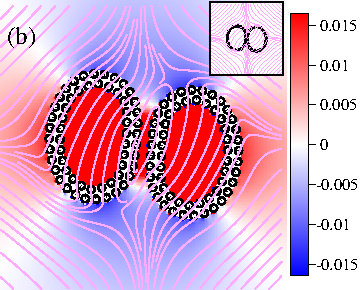
\includegraphics[height=2in]{N116_ext_2000.pdf}\\
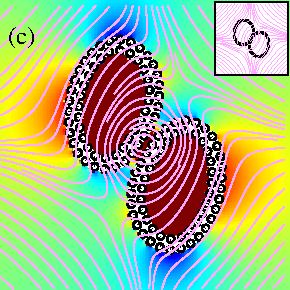
\includegraphics[height=2in]{N116_ext_4000.pdf}
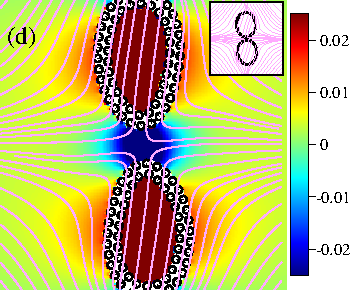
\includegraphics[height=2in]{N116_ext_6500.pdf}
  \caption{\label{figure12} Two JP vesicles suspended in an
  extensional flow where the dimensioneless extensional rate is
  $\chi=0.005$. The centroid of the left JP vesicle is $0.1$ units
  above the $x$-axis and the centroid of the right JP vesicle is
  $0.1$ units below the $x$-axis. The initial configuration is shown in
  panel (a). The background color is the fluid pressure. The color bar
  is identical for all panels. Streamlines are plotted in purple. The
  insets of all panels are generated from simulations of a continuum
  model of the vesicles and the streamlines agree between the models.}
\end{figure}





%%%%%%%%%%%%%%%%%%%%%%%%%%%%%%%%%%%%%%%%%%%%%%%%%%%%%%%%%%%%%%%%%%%%%%%
\subsubsection{Extensional Flow}

Using a similar setup to the shear case, we suspend the same two
pre-relaxed $58$-body JP vesicles and consider their dynamics in an
extensional flow with extensional rate $\chi=0.005$. This extensional
flow is stretching in the $y$ direction and squeezing in the $x$
direction. Figure~\ref{figure11} shows how the initial placement of the
JP vesicles affects the dynamics. When two centroids are both placed
symmetrically on the $x$-axis (case (i)), the JP vesicles reach a steady
equilibrium. If one centroid is placed above the $x$-axis (case (ii)),
the two JP vesicle move together and then upward. The migration of the
right JP vesicle is a consequence of the adhesive effect caused by the
hydrophobic interactions. When the two centroids start on opposite sides
of the $x$-axis (case (iii)), they eventually diverge from one another
along the $\pm y$-directions. Finally, when the two centroids start on
opposite sides of the $x$-axis, but with a greater displacement (case
(iv)), the JP vesicles move much faster along the $\pm y$-directions.

Figure~\ref{figure12} shows numerical results when the centroids of the
two Janus particles are placed at $(-10,-0.1)$ and $(10,0.1)$ (case
(iii) from Figure~\ref{figure11}). With this setup, the two JP vesicles
eventually separate along the $\pm y$-directions and we compare the
results against a continuum model as shown in all insets. Panels
(b)--(d) show the transient behavior of the JP vesicles and the
continuum vesicles under an extensional flow. In both the coarse-grained
model and the continuum model, the vesicles initially converge towards
one other and then diverge along the $y$-axis. The behavior of the
streamlines in both cases are similar. The pressure is initially largest
in the gap formed by two JP vesicles and decreases during the
separation. The short range repulsion plays an important role to avoid
structure collisions.
%and this result can be
%compared with some findings in continuum modeling simulations. 

%may need to add more here



%%%%%%%%%%%%%%%%%%%%%%%%%%%%%%%%%%%%%%%%%%%%%%%%%%%%%%%%%%%%%%%%%%%%%%%
\section{\label{conclusion}Conclusion}




This study proposes a continuum coarse-grained model for JP vesicle that focuses on the 
hydrophobic interactions between lipids and hydrodynamic interactions.
The mobility problem using integral equation methods combines the previously introduced HAP and the 
revised hydrophobic force for obtaining particle dynamics. 



The imposed forces and torques of JP system adopt not only HAP but also a newly developed short 
range repulsion given by \ref{eq:REPULforce} and \ref{eq:REPULtorque}.
The hydrodynamic stress tensor calculated in the algorithm leads to examinations of permeable 
membrane where the stretching modulus $K_A$ and the permeability constant $P$ can be obtained.
%
With the use of selected parameters, the numerical algorithm yields good qualitative results such as
phenomena in tank-treading JP vesicle. The reduced area $A^*$ decreases as the shear rate increases
 and we measure the equilibrium reduced area for a number of shear rates. The results show that the total
 length of JP vesicle is conserved and the decay rate of the reduced area is independent of shear rates when shear rates $\dot\gamma$ are between $\sim0.005$ ns$^{-1}$ and $0.008$ ns$^{-1}$.
Moreover, the proposed model can capture the membrane rupture when the shear flow is at a high shear rate
and this makes a breakthrough about having an idea for simulating such phenomenon different from other continuum modeling simulations when the bilayer membrane is represented as a closed and continuous curve.


Inter-monolayer friction coefficients $b$ are then obtained and reported by calculating the friction force $F_f$
using pressure jumps and slip velocities with respect to the bilayer midplane.
The resulting friction coefficients $b$ are about one order of magnitude smaller than ones in
~\cite{denOtter2007} and this observation suggests that the granularity of the system is a factor of having 
the discrepancy. The coarse-graining level of the JP vesicle has much longer length scale comparing against
the molecular dynamics simulations, in addition, the repulsive potential creates gaps between JP where the 
error in slip velocities piles up over the computational time.



We also study the migration of a JP vesicle suspended in a parabolic flow and obtain the asymmetric slipper shape. The reduced area $A^*$ of the starting JP vesicle is closed to 1 and $A^*=0.9$ at the equilibrium
state. A qualitative agreement has been made comparing with the two-dimensional inextensible membrane in continuum modeling simulations presented in~\cite{Kaoui09}. An interesting outcome is that the mean
$y$-position of the JP vesicle performs an oscillatory motion toward the center of the Poiseuille flow and this
may be caused by the granularity of the JP vesicle and choices of model parameters.


Results of two JP vesicles suspended in both shear and extensional flows have outstanding agreements with ones generated using continuum modeling in streamlines comparisons.
For two JP vesicles in shear flow, a demonstration of rotating behavior is presented and two overlapping 
trajectories of two centroid are observed as expected when two starting centroids are placed on the same 
horizontal level. The hydrophobic action and the repulsive potential lead to an adhesive effect when two 
JP bilayers are within a short distance.
We provide a series of results when two JP vesicles are suspended in extensional flow. We obtain similar results to the ones in \cite{qua-vee-you2019} when the reduced area $A^*$ is high and both centroids are placed 
with some vertical displacements.



Our future goal is to extend the current framework to a three-dimensional JP vesicle system. 
The further implementation of adding a fast algorithms such as the fast multipole method is also a 
practical approach.
Having a more physical boundary conditions on JP boundaries with experimental data is a reasonable direction and the future comparison with the laboratory experiments can be accomplished.







\begin{acknowledgments}
%We would like to acknowledge 
\end{acknowledgments}

%\appendix
%
%\section{Appendices}
%\label{sec:appendixA}

\bibliographystyle{jfm}
\bibliography{reference}% Produces the bibliography via BibTeX.





%\bibliographystyle{jfm}
%\bibliography{jfm}
%Use of the above commands will create a bibliography using the .bib file. Shown below is a bibliography built from individual items.


%\bibliography{jfm2esam}

%\begin{thebibliography}{99}
%
%\expandafter\ifx\csname natexlab\endcsname\relax
%\def\natexlab#1{#1}\fi
%\expandafter\ifx\csname selectlanguage\endcsname\relax
%\def\selectlanguage#1{\relax}\fi
%
%\bibitem[Batchelor (1971)]{Batchelor59}
%{\sc Batchelor, G.K.} 1971 {Small-scale variation of convected quantities like temperature in turbulent fluid part1, general discussion and the case of small conductivity}, {\it J. Fluid Mech.}, {\bf 5}, pp. 3-113-133.
%
%\bibitem [Bouguet (2008)]{Bouguet01}
%{\sc Bouguet, J.-Y} 2008 Camera Calibration Toolbox for Matlab {\url{http://www.vision.caltech.edu/bouguetj/calib_doc/}}.
%
% \bibitem[Briukhanovetal et al (1967)] {Briukhanovetal1967}
%{\sc Briukhanov, A. V.,   Grigorian, S. S., Miagkov,  S. M., Plam, M. Y.,   I. E. Shurova, I. E.,   Eglit, M. E. and Yakimov, Y. L.} 1967
%{On some new approaches to the dynamics of snow avalanches},
%{\it Physics of Snow and Ice,  Proceedings of the International Conference on Low Temperature Science}
%{Vol 1} pp. 1221--1241 {Institute of Low Temperature Science, Hokkaido University, Sapporo, Hokkaido, Japan}.
%
%\bibitem[Brownell (2004)]{Brownell04}
% {\sc Brownell,  C.J.  and Su,  L.K.} 2004  {Planar measurements of differential diffusion in turbulent jets}, {\it AIAA Paper},  pp. 2004-2335.
%
%\bibitem[Brownell and Su (2007)] {Brownell07}
%  {\sc Brownell, C.J. and  Su, L.K.} 2007 {Scale relations and spatial spectra in a differentially diffusing jet}, {\it AIAA Paper}, pp 2007-1314.
%
%\bibitem [Dennis (1985)] {Dennis85}
% {\sc  Dennis, S.C.R.} 1985 {Compact explicit finite difference approximations to the Navier--Stokes equation},  { In \it Ninth Intl Conf. on Numerical Methods in Fluid Dynamics},  {ed Soubbaramayer and J.P. Boujot},  {Vol 218}, {\it Lecture Notes in Physics}, pp. 23-51. Springer.
%
%\bibitem [Edwards et al. (2017)]{EdwardsVirouletKokelaarGray2017}
%{\sc Edwards, A. N., Viroulet, S., Kokelaar, B. P. and Gray, J. M. N. T.} 2017 Formation of levees, troughs and elevated channels by avalanches on erodible slopes {\it J. Fluid Mech.}, {\bf 823}, pp. 278-315.
%
%\bibitem[Hwang et al (1970)] {Hwang70}
% {\sc Hwang,  L.-S.  and  Tuck, E.O.} 1970 On the oscillations of harbours of arbitrary shape {\it J.~Fluid Mech.}, {\bf42}, pp 447-464.
%
%\bibitem[Josep and Saut (1990)] {JosephSaut1990}
% {\sc Joseph, Daniel D. and Saut, Jean Claude} 1990 Short-wave instabilities and ill-posed initial-value problems {\it Theoretical and Computational Fluid Dynamics}, {\bf 1},  pp.191--227,  {\url{http://dx.doi.org/10.1007/BF00418002}}.
%
%\bibitem[Worster (1992)] {Worster92}
%{ \sc  Worster, M.G.} 1992 The dynamics of mushy layers {\it Interactive dynamics of convection and solidification},
%{(ed. S.H. Davis and H.E. Huppert and W. Muller and M.G. Worster)}, pp. 113--138 {Kluwer}.
%
%\bibitem[Koch(1983)] {Koch83}
%{\sc Koch, W.} 1983 Resonant acoustic frequencies of flat plate cascades {\it J.~Sound Vib.}, {\bf 88}, pp. 233-242.
%
%\bibitem[Lee(1971)] {Lee71}
%{\sc Lee,  J.-J.}  1971 Wave-induced oscillations in harbours of arbitrary geometry {\it J.~Fluid Mech.}, {\bf 45}, pp. 375-394.
%
%\bibitem[Linton and  Evans (1992)] {Linton92}
% {\sc  Linton, C.M. and  Evans, D.V.} 1992 The radiation and scattering of surface waves by a vertical circular cylinder in a channel {\it Phil.\ Trans.\ R. Soc.\ Lond.}, {\bf 338}, pp. 325-357.
%
%\bibitem [Martin(1980] {Martin80}
% {\sc  Martin, P.A.} 1980 On the null-field equations for the exterior problems of acoustics {\it Q.~J. Mech.\ Appl.\ Maths},{\bf 33}, pp. 385--396.
%
%\bibitem [Rogallo(1981)] {Rogallo81}
% {\sc Rogallo,  R.S.} 1981 Numerical experiments in homogeneous turbulence  { {\it Tech. Rep.} 81835}  {NASA Tech.\ Mem}.
%
%\bibitem[Ursell(1950)] {Ursell50}
%{\sc  Ursell, F.} 1950 Surface waves on deep water in the presence of a submerged cylinder i {\it Proc.\ Camb.\ Phil.\ Soc.}, {\bf 46}, pp.141--152.
%
%\bibitem[Wijngaarden (1968)]{Wijngaarden68}
%{\sc van Wijngaarden, L.} 1968 On the oscillations Near and at resonance in open pipes {\it J.~Engng Maths},{\bf 2}, pp. 225--240.
%
%\bibitem[Miller (1991)]{Miller91}
%{ \sc  Miller, P.L.} 1991 Mixing in high Schmidt number turbulent jets {school {PhD thesis}} {California Institute of Technology}.
%
%\end{thebibliography}

%% End of file `jfm2esam.bib'.

\end{document}
